\documentclass{vkr}
\usepackage[english, russian]{babel} % переносы
\usepackage{graphicx} % для вставки картинок
\graphicspath{{images/}} % путь к изображениям
\usepackage[hidelinks]{hyperref}
\usepackage{float} % определяет метод H для рисунка с переносом на следующую страницу, ели не помещается
\usepackage{pdflscape}
\addto{\captionsrussian}{\renewcommand{\refname}{СПИСОК ИСПОЛЬЗОВАННЫХ ИСТОЧНИКОВ}}
\usepackage{xltabular} % для вставки таблиц
\usepackage{makecell}
\renewcommand\theadfont{} % шрифт в /thead
\usepackage{array} % для определения новых типов столбцов таблиц
\newcolumntype{T}{>{\centering\arraybackslash}X} % новый тип столбца T - автоматическая ширина столбца с выравниванием по центру
\newcolumntype{R}{>{\raggedleft\arraybackslash}X} % новый тип столбца R - автоматическая ширина столбца с выравниванием по правому краю
\newcolumntype{C}[1]{>{\centering\let\newline\\\arraybackslash\hspace{0pt}}m{#1}} % новый тип столбца C - фиксированная ширина столбца с выравниванием по центру
\newcolumntype{r}[1]{>{\raggedleft\arraybackslash}p{#1}} % новый тип столбца r - фиксированная ширина столбца с выравниванием по правому краю
\newcommand{\centrow}{\centering\arraybackslash} % командой \centrow можно центрировать одну ячейку (заголовок) в столбце типа X или p, оставив в оcтальных ячейках другой тип выравнивания
\newcommand{\finishhead}{\endhead\hline\endlastfoot}
\newcommand{\continuecaption}[1]{\captionsetup{labelformat=empty} \caption[]{#1}\\ \hline }
\usepackage{etoolbox}
\AtBeginEnvironment{xltabular}{\refstepcounter{tablecnt}} % подсчет таблиц xltabular, обычные таблицы подсчитываются в классе

\usepackage[tableposition=top]{caption} % подпись таблицы вверху
\captionsetup{strut=off}
\setlength{\intextsep}{0pt} % Vertical space above & below [h] floats
\setlength{\textfloatsep}{0pt} % Vertical space below (above) [t] ([b]) floats
\DeclareCaptionLabelFormat{gostfigure}{Рисунок #2} %подпись рисунка
\DeclareCaptionLabelFormat{gosttable}{Таблица #2} %подпись таблицы
\DeclareCaptionLabelSeparator{gost}{~--~} %разделитель в рисунках и таблицах
\captionsetup{labelsep=gost}
\captionsetup[figure]{aboveskip=10pt,belowskip=4mm,justification=centering,labelformat=gostfigure} % настройка подписи рисунка
\captionsetup[table]{font={stretch=1.41},skip=0pt,belowskip=0pt,aboveskip=8.5pt,singlelinecheck=off,labelformat=gosttable} % настройка подписи таблицы

\setlength{\LTpre}{8mm} % отступ сверху таблицы
\setlength{\LTpost}{6mm} % отступ снизу таблицы

\usepackage{enumitem}
%\renewcommand{\labelitemi}{\textbullet} % Вернёт стандартные точки
\setlist{nolistsep,wide=\parindent,itemindent=*} % отступы вокруг списков, выравнивание с учетом разделителя

\usepackage{color} %% это для отображения цвета в коде
\usepackage{listings} %% листинги кода
\setmonofont[Scale=0.7]{Verdana} % моноширный шрифт для листинга

\definecolor{codegreen}{rgb}{0,0.6,0}
\definecolor{codegray}{rgb}{0.5,0.5,0.5}
\definecolor{codepurple}{rgb}{0.58,0,0.82}

\lstset{ %
language=C,                 % выбор языка для подсветки (здесь это С)
numbers=left,               % где поставить нумерацию строк (слева\справа)
numberstyle=\tiny,           % размер шрифта для номеров строк
stepnumber=1,                   % размер шага между двумя номерами строк
numbersep=5pt,                % как далеко отстоят номера строк от подсвечиваемого кода
commentstyle=\color{codegreen},
keywordstyle=\color{magenta},
numberstyle=\tiny\color{codegray},
stringstyle=\color{codepurple},
basicstyle=\linespread{0.95}\ttfamily,
backgroundcolor=\color{white}, % цвет фона подсветки - используем \usepackage{color}
showspaces=false,            % показывать или нет пробелы специальными отступами
showstringspaces=false,      % показывать или нет пробелы в строках
showtabs=false,             % показывать или нет табуляцию в строках
frame=single,              % рисовать рамку вокруг кода
tabsize=2,                 % размер табуляции по умолчанию равен 2 пробелам
captionpos=t,              % позиция заголовка вверху [t] или внизу [b] 
breaklines=true,           % автоматически переносить строки (да\нет)
breakatwhitespace=false, % переносить строки только если есть пробел
escapeinside={\%*}{*)}   % если нужно добавить комментарии в коде
}

\makeatletter % чтобы допускались русские комментарии в листингах
\lst@InputCatcodes
\def\lst@DefEC{%
 \lst@CCECUse \lst@ProcessLetter
  ^^80^^81^^82^^83^^84^^85^^86^^87^^88^^89^^8a^^8b^^8c^^8d^^8e^^8f%
  ^^90^^91^^92^^93^^94^^95^^96^^97^^98^^99^^9a^^9b^^9c^^9d^^9e^^9f%
  ^^a0^^a1^^a2^^a3^^a4^^a5^^a6^^a7^^a8^^a9^^aa^^ab^^ac^^ad^^ae^^af%
  ^^b0^^b1^^b2^^b3^^b4^^b5^^b6^^b7^^b8^^b9^^ba^^bb^^bc^^bd^^be^^bf%
  ^^c0^^c1^^c2^^c3^^c4^^c5^^c6^^c7^^c8^^c9^^ca^^cb^^cc^^cd^^ce^^cf%
  ^^d0^^d1^^d2^^d3^^d4^^d5^^d6^^d7^^d8^^d9^^da^^db^^dc^^dd^^de^^df%
  ^^e0^^e1^^e2^^e3^^e4^^e5^^e6^^e7^^e8^^e9^^ea^^eb^^ec^^ed^^ee^^ef%
  ^^f0^^f1^^f2^^f3^^f4^^f5^^f6^^f7^^f8^^f9^^fa^^fb^^fc^^fd^^fe^^ff%
  ^^^^20ac^^^^0153^^^^0152%
  % Basic Cyrillic alphabet coverage
  ^^^^0410^^^^0411^^^^0412^^^^0413^^^^0414^^^^0415^^^^0416^^^^0417%
  ^^^^0418^^^^0419^^^^041a^^^^041b^^^^041c^^^^041d^^^^041e^^^^041f%
  ^^^^0420^^^^0421^^^^0422^^^^0423^^^^0424^^^^0425^^^^0426^^^^0427%
  ^^^^0428^^^^0429^^^^042a^^^^042b^^^^042c^^^^042d^^^^042e^^^^042f%
  ^^^^0430^^^^0431^^^^0432^^^^0433^^^^0434^^^^0435^^^^0436^^^^0437%
  ^^^^0438^^^^0439^^^^043a^^^^043b^^^^043c^^^^043d^^^^043e^^^^043f%
  ^^^^0440^^^^0441^^^^0442^^^^0443^^^^0444^^^^0445^^^^0446^^^^0447%
  ^^^^0448^^^^0449^^^^044a^^^^044b^^^^044c^^^^044d^^^^044e^^^^044f%
  ^^^^0401^^^^0451%
  %%%
  ^^00}
\lst@RestoreCatcodes
\makeatother


% Режим шаблона (должен быть включен один из трех)
% \ВКРtrue
\Практикаtrue
%\Курсоваяtrue

\newcommand{\Дисциплина}{<<Проектирование и архитектура программных систем>>} % для курсовой
\newcommand{\КодСпециальности}{09.03.04} % Курсовая
\newcommand{\Специальность}{Программная инженерия} % Курсовая
\newcommand{\Тема}{Разработка веб-платформы для автоматизации бизнес-процессов управления персоналом компании} % ВКР Курсовая
\newcommand{\ТемаВтораяСтрока}{1С-Битрикс}
\newcommand{\ГдеПроводитсяПрактика}{ООО <<Предприятие ВТИ-Сервис>>} % для практики
\newcommand{\РуководительПрактПредпр}{Федосов Д. В.} % для практики
\newcommand{\ДолжнРуководительПрактПредпр}{директор} % для практики
\newcommand{\РуководительПрактУнивер}{Чаплыгин А. А.} % для практики
\newcommand{\ДолжнРуководительПрактУнивер}{к.т.н. доцент} % для практики
\newcommand{\Автор}{П. В. Орлов}
\newcommand{\АвторРод}{Орлова П.В.}
\newcommand{\АвторПолностьюРод}{Орлова Павла Вадимовича} % для практики
\newcommand{\Шифр}{21-06-0124}
\newcommand{\Курс}{4 } % для практики
\newcommand{\Группа}{ПО-11б}
\newcommand{\Руководитель}{А. А. Чаплыгин} % для ВКР и курсовой
\newcommand{\Нормоконтроль}{А. А. Чаплыгин} % для ВКР
\newcommand{\ЗавКаф}{А. В. Малышев} % для ВКР
\newcommand{\ДатаПриказа}{«07» апреля 2023~г.} % для ВКР
\newcommand{\НомерПриказа}{1505-с} % для ВКР
\newcommand{\СрокПредоставления}{«13» июня 2023~г.} % для ВКР, курсового

\begin{document}
\maketitle
\ifПрактика{}\else{
   \newpage
\begin{center}
\large\textbf{Минобрнауки России}

\large\textbf{Юго-Западный государственный университет}
\vskip 1em
\normalsize{Кафедра программной инженерии}
\vskip 1em
\ifВКР{
        \begin{flushright}
        \begin{tabular}{p{.4\textwidth}}
        \centrow УТВЕРЖДАЮ: \\
        \centrow Заведующий кафедрой \\
        \hrulefill \\
        \setarstrut{\footnotesize}
        \centrow\footnotesize{(подпись, инициалы, фамилия)}\\
        \restorearstrut
        «\underline{\hspace{1cm}}»
        \underline{\hspace{3cm}}
        20\underline{\hspace{1cm}} г.\\
        \end{tabular}
        \end{flushright}
        }\fi
\end{center}
\vspace{1em}
  \begin{center}
  \large
\ifВКР{
ЗАДАНИЕ НА ВЫПУСКНУЮ КВАЛИФИКАЦИОННУЮ РАБОТУ
  ПО ПРОГРАММЕ БАКАЛАВРИАТА}
  \else
ЗАДАНИЕ НА КУРСОВУЮ РАБОТУ (ПРОЕКТ)
\fi
\normalsize
  \end{center}
\vspace{1em}
{\parindent0pt
  Студента \АвторРод, шифр\ \Шифр, группа \Группа
  
1. Тема «\Тема\ \ТемаВтораяСтрока»
\ifВКР{
утверждена приказом ректора ЮЗГУ от \ДатаПриказа\ № \НомерПриказа
}\fi.

2. Срок предоставления работы к защите \СрокПредоставления

3. Исходные данные для создания программной системы:

3.1. Перечень решаемых задач:}

\renewcommand\labelenumi{\theenumi)}

\begin{enumerate}
\item Проанализировать IT-инфраструктуру предприятия.
\item Разработать концептуальную модель системы управления IT-ин\-фра\-струк\-турой предприятия на основе подхода к управлению и организации ИТ-услуг ITSM.
\item Спроектировать программную систему управления IT-ин\-фра\-струк\-турой предприятия.
\item Сконструировать и протестировать программную систему управления IT-инфраструктурой предприятия.
\end{enumerate}

{\parindent0pt
  3.2. Входные данные и требуемые результаты для программы:}

\begin{enumerate}
\item Входными данными для программной системы являются: данные справочников комплектующих, конфигураций, ПО, критериев качества SLA, ИТ-услуг, департаментов компании; технические данные ИТ-ресурсов; данные входящих заявок на ИТ-ресурсы; данные запросов поставщикам на комплектующие.
\item Выходными данными для программной системы являются: сформированные заявки на обслуживание ИТ-ресурсов; сформированные запросы на закупку комплектующих; сведения о выполненных работах по заявкам; статусы заявок; выходные отчеты (инфографика) – по качеству услуг, по состоянию ИТ-ресурсов, по деятельности ИТ-отдела, по стоимости обслуживания ИТ-ресурсов, воронка заявок.
\end{enumerate}

{\parindent0pt

  4. Содержание работы (по разделам):
  
  4.1. Введение.
  
  4.1. Анализ предметной области.
  
4.2. Техническое задание: основание для разработки, назначение разработки,
требования к программной системе, требования к оформлению документации.

4.3. Технический проект: общие сведения о программной системе, проект
данных программной системы, проектирование архитектуры программной системы, проектирование пользовательского интерфейса программной системы.

4.4. Рабочий проект: спецификация компонентов и классов программной системы, тестирование программной системы, сборка компонентов программной системы.

4.5. Заключение.

4.6. Список использованных источников.

5. Перечень графического материала:

\списокПлакатов

\vskip 2em
\begin{tabular}{p{6.8cm}C{3.8cm}C{4.8cm}}
Руководитель \ifВКР{ВКР}\else работы (проекта) \fi & \lhrulefill{\fill} & \fillcenter\Руководитель\\
\setarstrut{\footnotesize}
& \footnotesize{(подпись, дата)} & \footnotesize{(инициалы, фамилия)}\\
\restorearstrut
Задание принял к исполнению & \lhrulefill{\fill} & \fillcenter\Автор\\
\setarstrut{\footnotesize}
& \footnotesize{(подпись, дата)} & \footnotesize{(инициалы, фамилия)}\\
\restorearstrut
\end{tabular}
}

\renewcommand\labelenumi{\theenumi.}

   \abstract{РЕФЕРАТ}

Объем работы равен \formbytotal{lastpage}{страниц}{е}{ам}{ам}. Работа содержит \formbytotal{figurecnt}{иллюстраци}{ю}{и}{й}, \formbytotal{tablecnt}{таблиц}{у}{ы}{}, \arabic{bibcount} библиографических источников и \formbytotal{числоПлакатов}{лист}{}{а}{ов} графического материала. Количество приложений – 2. Графический материал представлен в приложении А. Фрагменты исходного кода представлены в приложении Б.

Перечень ключевых слов: веб-платформа, веб-сайт, автоматизация, управление персоналом, PWA, бизнес-процессы, TypeScript, React, JMAP, почта, мессенджер, видеоконференцсвязь, SMTP, JSON, DOM, интерфейс, навигация.

Объектом разработки является веб-платформа для автоматизации управления персоналом компании, включающая модули для работы с почтой, задачами, календарем, видеоконференциями, файлами и контактами.

Целью выпускной квалификационной работы является разработка и внедрение веб-платформы, обеспечивающей эффективное управление внутренними коммуникациями и координацией персонала компании. Платформа призвана решить проблемы фрагментированности бизнес-сервисов, неэффективной коммуникации между сотрудниками и отсутствия единой системы хранения информации.

В процессе создания платформы была разработана концептуальная модель системы, в результате которой спроектирован пользовательский интерфейс и структура данных вместе с архитектурой платформы, внедрены модули для сервисов. 

Разработанная платформа была успешно внедрена в компании АО «Белуга Проджектс Лоджистик».

\selectlanguage{english}
\abstract{ABSTRACT}
  
The volume of work is \formbytotal{lastpage}{page}{}{s}{s}. The work contains \formbytotal{figurecnt}{illustration}{}{s}{s}, \formbytotal{tablecnt}{table}{}{s}{s}, \arabic{bibcount} bibliographic sources and \formbytotal{числоПлакатов}{sheet}{}{s}{s} of graphic material. The number of applications is 2. The graphic material is presented in annex A. The layout of the site, including the connection of components, is presented in annex B.

List of keywords: web platform, website, automation, HR management, PWA, business processes, TypeScript, React, JMAP, mail, messenger, video conferencing, SMTP, JSON, DOM, interface, navigation.

The development object is a web platform for automating the management of company personnel, including modules for working with mail, tasks, calendar, video conferences, files and contacts.

The purpose of the final qualification work is to develop and implement a web platform that ensures effective management of internal communications and coordination of the company's personnel. The platform is designed to solve the problems of fragmentation of business services, ineffective communication between employees and the lack of a unified information storage system.

During the process of creating the platform, a conceptual model of the system was developed, as a result of which the user interface and data structure were designed together with the platform architecture, and modules for services were implemented.

The developed platform was successfully implemented in the company JSC Beluga Projects Logistics.
\selectlanguage{russian}
}\fi
\tableofcontents
\section*{ОБОЗНАЧЕНИЯ И СОКРАЩЕНИЯ}

БД -- база данных.

ИС -- информационная система.

ИТ -- информационные технологии. 

КТС -- комплекс технических средств.

ОМТС -- отдел материально-технического снабжения. 

ПО -- программное обеспечение.

РП -- рабочий проект.

СУБД -- система управления базами данных.

ТЗ -- техническое задание.

ТП -- технический проект.

UML (Unified Modelling Language) -- язык графического описания для объектного моделирования в области разработки программного обеспечения.

ВКС -- видеоконференцсвязь

\ifПрактика{}\else{\section*{ВВЕДЕНИЕ}
\addcontentsline{toc}{section}{ВВЕДЕНИЕ}

Современные предприятия сталкиваются с необходимостью повышения эффективности внутренних процессов, улучшения коммуникации между сотрудниками и централизации бизнес-сервисов. В условиях цифровой трансформации особую актуальность приобретает автоматизация управления персоналом — ключевого ресурса любой организации.

Традиционно компании используют множество разрозненных решений: почтовые клиенты, мессенджеры, системы управления задачами, календари, сервисы видеосвязи и облачные хранилища. Отсутствие единого интерфейса и централизованного подхода к управлению такими сервисами приводит к фрагментированности данных, росту временных затрат и снижению продуктивности сотрудников.

Для решения указанных проблем в данной работе разрабатывается универсальная веб-платформа, объединяющая основные модули для эффективной организации внутренних коммуникаций и управления задачами внутри компании. Платформа реализована с использованием современных веб-технологий, таких как TypeScript, React, JMAP, и представляет собой прогрессивное веб-приложение (PWA) с модульной архитектурой.

Разработка охватывает создание сервисов: электронной почты, календаря, контактов, файлового хранилища, видеоконференций, чатов, панели управления и системы управления проектами. Все компоненты взаимосвязаны и доступны через единый пользовательский интерфейс.

\emph{Цель настоящей работы} — разработка и внедрение веб-платформы, обеспечивающей автоматизацию бизнес-процессов управления персоналом, повышение прозрачности взаимодействия и улучшение координации в рамках одного цифрового пространства.

Для достижения поставленной цели необходимо решить следующие \emph{задачи:}
\begin{itemize}
\item провести анализ предметной области и существующих решений;
\item разработать концептуальную модель веб-платформы;
\item спроектировать архитектуру платформы и пользовательский интерфейс;
\item реализовать модули платформы с применением современных технологий;
\item провести тестирование готовой системы и внедрить её в организацию.
\end{itemize}

\emph{Структура и объём работы.} Отчет состоит из введения, четырёх разделов основной части, заключения, списка использованных источников и двух приложений. Общий объем текста составляет \formbytotal{lastpage}{страниц}{у}{ы}{}. Работа содержит графический материал (приложение А) и исходный код (приложение Б).

\emph{Во введении} обозначены цель, задачи и структура работы.

\emph{Первый раздел} посвящён анализу предметной области и описанию проблем, решаемых разрабатываемой системой.

\emph{Второй раздел} содержит техническое задание: формулируются требования к функциональности платформы, интерфейсу и архитектуре.

\emph{Третий раздел} включает проектные решения: выбор технологий, диаграммы компонентов, структура базы данных и описание взаимодействий.

\emph{Четвёртый раздел} содержит описание реализации, модульного и системного тестирования платформы.

В заключении подведены итоги работы и сделаны выводы по результатам внедрения платформы.

В приложении А представлен графический материал.
В приложении Б представлены фрагменты исходного кода. 
}\fi
\section{Анализ предметной области}
\subsection{Характеристика предприятия и его деятельности}

Компания \textbf{BELUGA TEC} — ведущий российский провайдер комплексных инжиниринговых и логистических решений для промышленных предприятий. Организация специализируется на проектировании и реализации грузоподъёмных, монтажных и транспортных операций на объектах нового строительства, действующих производств, капитального ремонта, модернизации и расширения производственных мощностей.

Основные направления деятельности компании включают:

\begin{enumerate}
  \item \textbf{Инжиниринг и монтажные работы}, охватывающие:
  \begin{itemize}
    \item проектирование и реализацию грузоподъёмных операций;
    \item монтаж негабаритного оборудования на различные высотные отметки;
    \item выполнение работ в стеснённых условиях без демонтажа несущих конструкций.
  \end{itemize}

  \item \textbf{Проектную логистику}, включающую:
  \begin{itemize}
    \item детальную проработку логистических схем;
    \item перемещение и подъём оборудования без остановки производства;
    \item альтернативные решения крановым операциям.
  \end{itemize}

  \item \textbf{Флот BELUGA Marine}, предоставляющий:
  \begin{itemize}
    \item морские транспортные услуги для доставки крупногабаритных грузов;
    \item специализированное подъёмное оборудование и транспортную технику.
  \end{itemize}

  \item \textbf{EPC/EPCM-проекты}, охватывающие:
  \begin{itemize}
    \item полный цикл инженерных и строительных услуг;
    \item управление проектами от концепции до ввода в эксплуатацию.
  \end{itemize}
\end{enumerate}

Компания активно работает в различных отраслях промышленности, включая:

\begin{itemize}
  \item нефтегазохимию;
  \item машиностроение;
  \item энергетику;
  \item горнодобывающую и обрабатывающую промышленность;
  \item металлургию;
  \item инфраструктурные проекты;
  \item порты и верфи.
\end{itemize}

\textbf{BELUGA TEC} внедряет инновационные технологии и уникальные технические решения, позволяющие:

\begin{itemize}
  \item снижать затраты за счёт применения бескрановых технологий подъёма;
  \item сокращать время монтажа при полной сборке оборудования на нулевой отметке;
  \item работать в условиях ограниченного пространства без демонтажа крыш цехов и нарушения теплового контура;
  \item минимизировать риски повреждения оборудования и несчастных случаев;
  \item учитывать природные зоны, особенности ландшафта и строительной площадки при выполнении работ.
\end{itemize}

С более чем 14-летним опытом на рынке и более 120 успешно реализованными проектами, \textbf{BELUGA TEC} зарекомендовала себя как надёжный партнёр в сфере комплексного инжиниринга и логистики для промышленных предприятий.


\subsection{Постановка задачи}

Для оптимизации внутренних процессов предприятия разрабатывается веб-платформа, направленная на автоматизацию управления персоналом. Основные проблемы, решаемые системой:

\begin{itemize}
  \item фрагментированность бизнес-сервисов;
  \item неэффективная коммуникация между сотрудниками;
  \item отсутствие единой системы хранения информации.
\end{itemize}

\subsection{Аналогичные решения и их анализ}

Среди известных решений на рынке выделяется Bitrix24.

Функции: CRM, управление проектами, задачи, календари, мессенджер, телефония, документы;

Достоинства: множество модулей в одном интерфейсе, интеграции с 1С и внешними API, развитый документооборот;

Недостатки: высокая стоимость при масштабировании, громоздкий интерфейс, избыточность для небольших компаний.


\subsection{Преимущества разрабатываемой системы}

Разрабатываемая веб-платформа предлагает:

\begin{itemize}
  \item единую точку входа к сервисам;
  \item централизованное управление пользователями и задачами;
  \item интуитивно понятный интерфейс;
  \item возможность расширения и интеграции;
  \item открытую архитектуру.
\end{itemize}

\subsection{Вывод}

Анализ предметной области и имеющихся решений показал, что разрабатываемая система будет актуальна для малого и среднего бизнеса, стремящегося к цифровой трансформации. Использование модульной архитектуры и современных технологий обеспечит гибкость, удобство и функциональную полноту, превосходящую отдельные существующие решения.
\section{Техническое задание}

\subsection{Основание для разработки}

Основанием для разработки является задание на выпускную квалификационную работу бакалавра <<Разработка веб-платформы для автоматизации бизнес-процессов управления персоналом компании>>. Проект реализуется в рамках производственной практики студента в компании ООО <<ВТИ-Сервис>>.

\subsection{Цель и назначение разработки}

Целью проекта является разработка и внедрение веб-платформы, которая обеспечит эффективное управление внутренними коммуникациями и координацией персонала.

Задачи разработки включают:

\begin{itemize}
  \item создание единого доступа ко всем внутренним бизнес-сервисам;
  \item централизация данных и снижение фрагментированности инструментов;
  \item повышение прозрачности процессов и контроль выполнения задач;
  \item ускорение документооборота и взаимодействия между сотрудниками;
  \item внедрение интуитивного интерфейса и адаптивной архитектуры.
\end{itemize}

\subsection{Функциональные задачи}

Разрабатываемая веб-платформа включает следующие сервисные модули:

  \textbf{Почта} — модуль для внутренней и внешней переписки. Реализует:
  \begin{itemize}
    \item просмотр и отправку писем;
    \item вложения и черновики;
    \item фильтрацию, сортировку и интеграцию с контактами.
  \end{itemize}

  \textbf{Контакты} — централизованная адресная книга:
  \begin{itemize}
    \item отображение статуса и информации о сотрудниках;
    \item быстрый доступ к действиям (сообщение, задача, звонок).
  \end{itemize}

  \textbf{Проекты} — система для постановки и отслеживания задач:
  \begin{itemize}
    \item создание задач и контроль сроков;
    \item фильтрация по статусу и исполнителям;
    \item иерархия задач и связь с календарём.
  \end{itemize}

  \textbf{Файлы} — облачное хранилище для документов:
  \begin{itemize}
    \item загрузка и скачивание;
    \item управление правами доступа;
    \item история изменений.
  \end{itemize}

  \textbf{Календарь} — модуль планирования событий:
  \begin{itemize}
    \item создание событий и напоминаний;
    \item интеграция с задачами и ВКС;
    \item уведомления о событиях.
  \end{itemize}

  \textbf{Разговоры} — встроенный мессенджер:
  \begin{itemize}
    \item чат с сотрудниками;
    \item групповые обсуждения;
    \item уведомления и синхронизация с почтой.
  \end{itemize}

  \textbf{ВКС} — видеоконференцсвязь:
  \begin{itemize}
    \item создание и участие во встречах;
    \item демонстрация экрана;
    \item чат во время звонков.
  \end{itemize}

  \textbf{Настройки} — модуль управления профилем:
  \begin{itemize}
    \item редактирование профиля;
    \item смена темы, языка;
    \item конфиденциальность.
  \end{itemize}

  \textbf{Панель управления} — стартовая страница с виджетами:
  \begin{itemize}
    \item отображение актуальных данных со всех сервисов;
    \item настройка отображаемых виджетов;
    \item персонализация интерфейса.
  \end{itemize}

\subsection{Требования пользователя к интерфейсу веб-платформы}

Интерфейс должен обеспечивать:
\begin{itemize}
  \item интуитивную навигацию между модулями;
  \item адаптивную вёрстку для десктопов и мобильных устройств;
  \item визуальное разграничение ролей пользователей;
  \item поддержку светлой и тёмной темы.
\end{itemize}

Композиция интерфейса сервиса <<Почта>> представлена на рисунке \ref{templ:image1} и состоит из:
\begin{itemize}
  \item кнопки для отправки письма(1);
  \item списка папок (2);
  \item окна для просмотра писем из выбранной папки (3);
  \item компонента пагинации (4);
  \item компонента навигации по сервисам (5);
\end{itemize}
\begin{figure}[H]
	\centering
	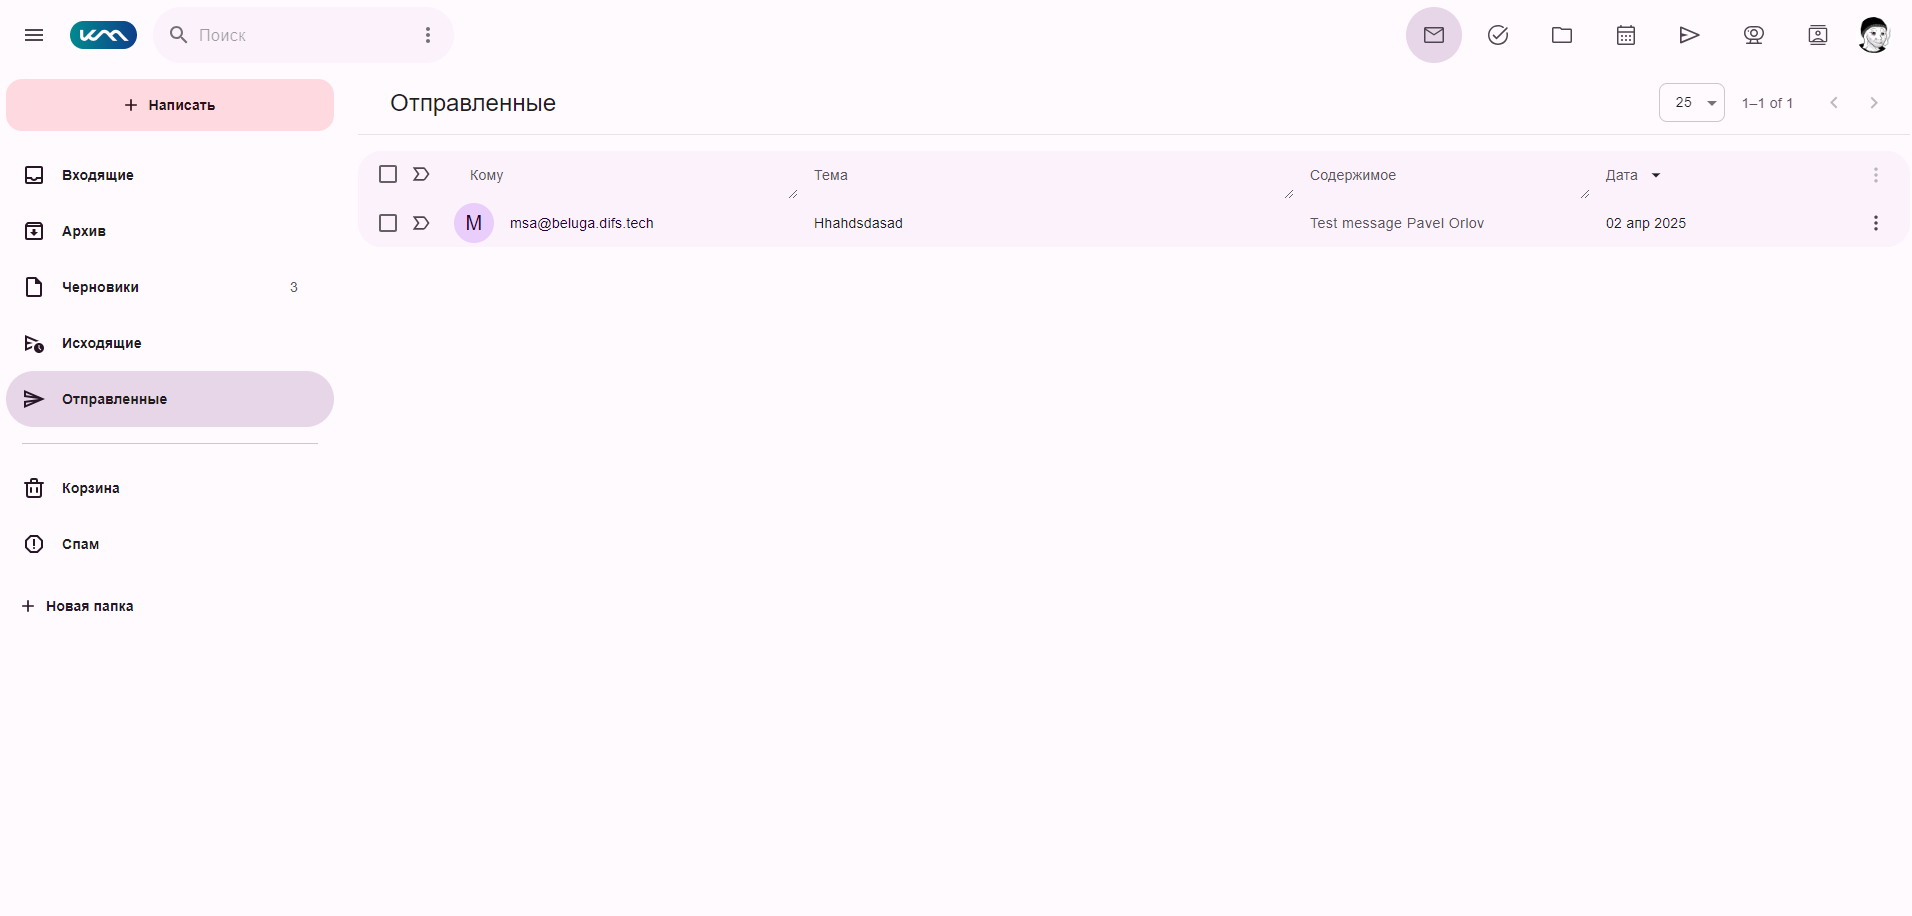
\includegraphics[width=1\linewidth]{images/почта}
	\caption{Композиция интерфейса сервиса <<Почта>>}
	\label{templ:image1}
\end{figure}

Композиция интерфейса написания письма в сервисе <<Почта>> представлена на рисунке \ref{templ:image1b} и состоит из:
\begin{itemize}
  \item окна ввода письма (1);
  \item поля ввода адресата (2);
  \item кнопок для ввода адресата с целью получения копии/скрытой копии (3);
  \item поля для ввода темы письма (4);
  \item окна для ввода тела письма (5);
  \item кнопок для отправки/сохранения письма в черновик (6);
  \item кнопок для прикрепления файла с компьютера или из сервиса <<Файлы>> (7);
  \item кнопки для закрытия окна без сохранения письма в черновик (8);
\end{itemize}
\begin{figure}[H]
	\centering
	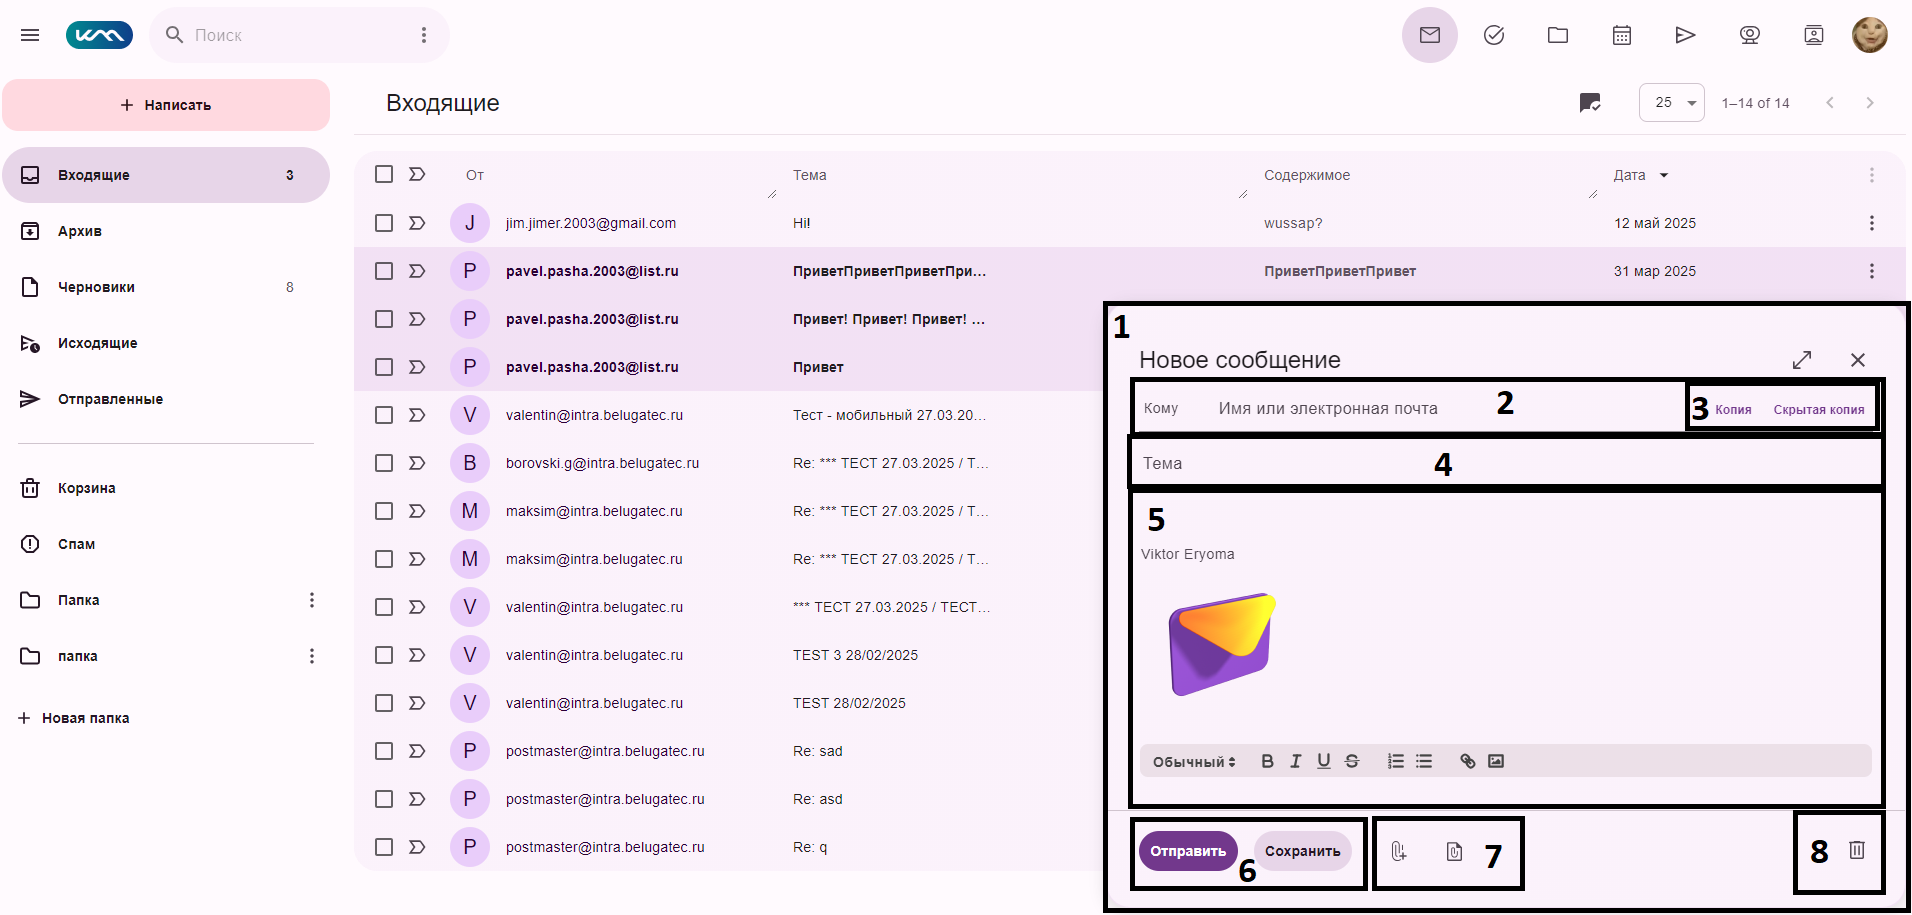
\includegraphics[width=1\linewidth]{images/почта2}
	\caption{Композиция интерфейса написания письма}
	\label{templ:image1b}
\end{figure}

Композиция интерфейса прикрепление файла из сервиса <<Файлы>> в сервисе <<Почта>> представлена на рисунке \ref{templ:image1c} и состоит из:
\begin{itemize}
  \item всплывающего окна(1);
  \item разделов с файлами (2);
  \item компонента файла с функцией выбора (3);
  \item кнопок для прикрепления файла (4);
\end{itemize}
\begin{figure}[H]
	\centering
	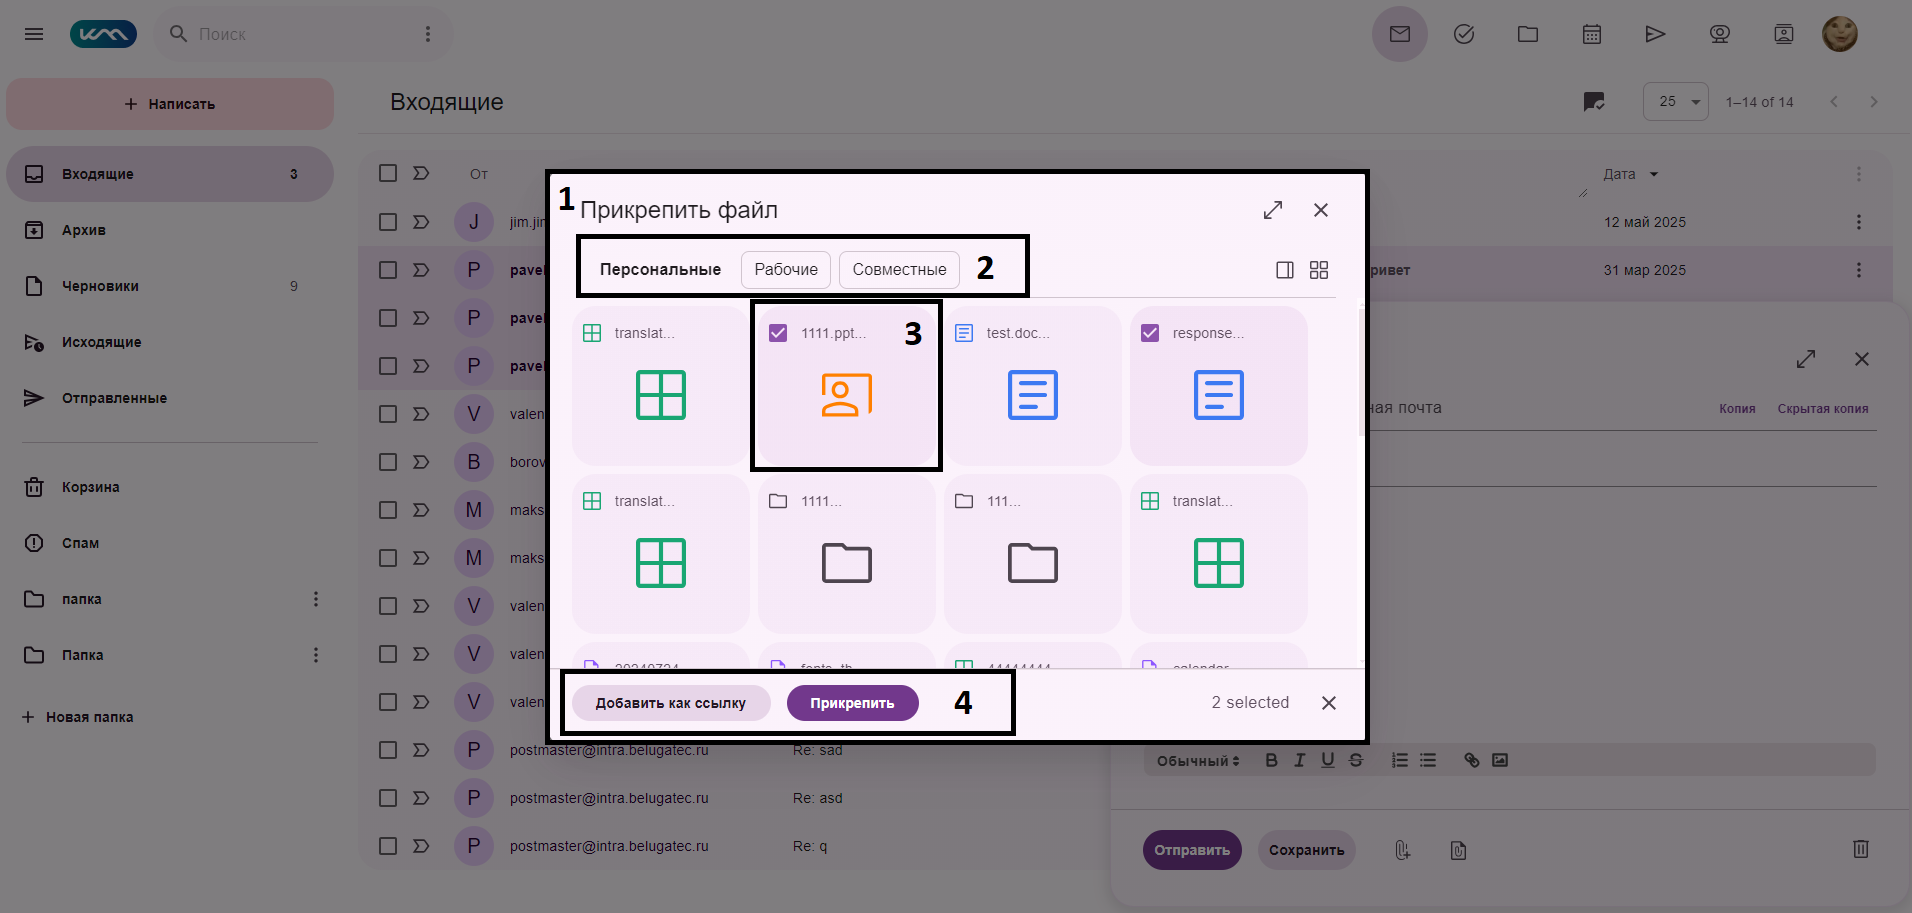
\includegraphics[width=1\linewidth]{images/почта3}
	\caption{Композиция интерфейса прикрепление файла}
	\label{templ:image1c}
\end{figure}

Композиция интерфейса создания папки в сервисе <<Почта>> представлена на рисунке \ref{templ:image1d} и состоит из:
\begin{itemize}
  \item всплывающего окна(1);
  \item поля ввода названия папки (2);
  \item кнопок действий (3);
\end{itemize}
\begin{figure}[H]
	\centering
	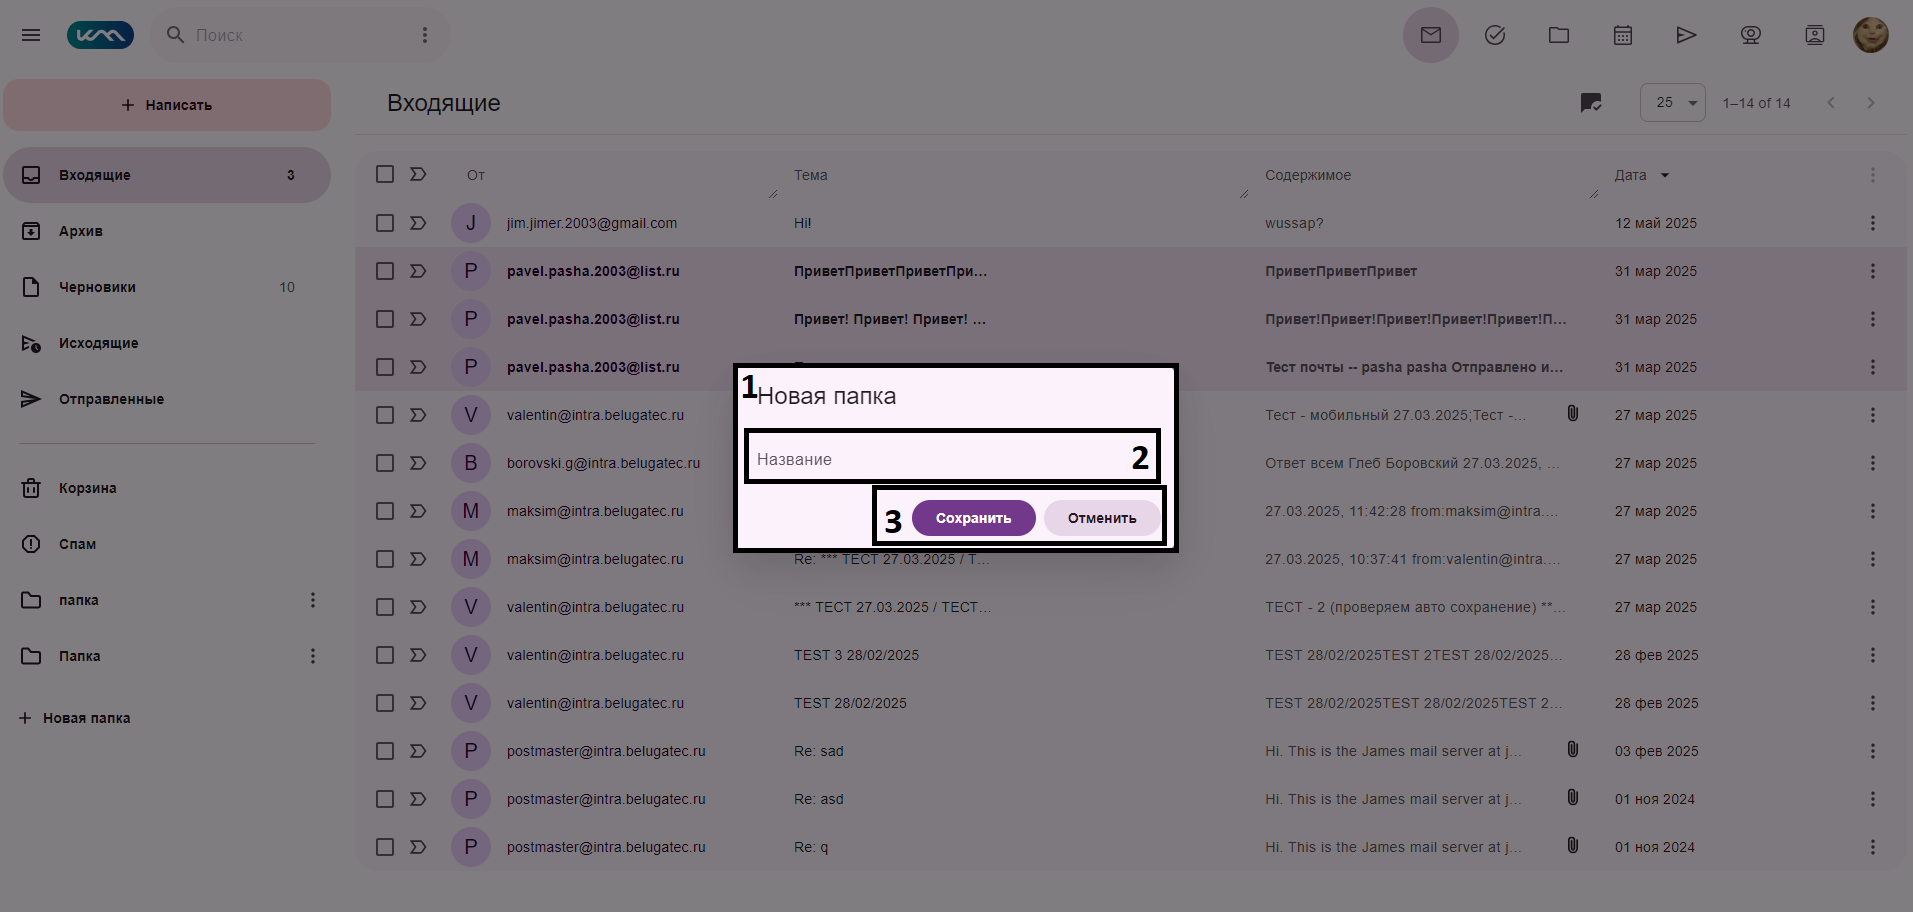
\includegraphics[width=1\linewidth]{images/почта4}
	\caption{Композиция интерфейса создания папки}
	\label{templ:image1d}
\end{figure}

Композиция интерфейса сервиса <<Видеоконференцсвязь>> представлена на рисунке \ref{templ:image2} и состоит из:
\begin{itemize}
  \item компонента навигации по сервисам (1);
  \item поля для ввода названия комнаты (2);
  \item кнопки для подключения к комнате (3);
  \item кнопки для подключения к запланированным встречам (4);
\end{itemize}
\begin{figure}[H]
	\centering
	
\includegraphics[width=1\linewidth]{images/вкс}
	\caption{Композиция интерфейса сервиса <<Видеоконференцсвязь>>}
	\label{templ:image2}
\end{figure}

Композиция интерфейса сервиса <<Календарь>> представлена на рисунке \ref{templ:image3} и состоит из:
\begin{itemize}
  \item компонента навигации по сервисам (1);
  \item кнопки для создания события (2);
  \item компонент уменьшенной версии календаря (3);
  \item кнопки фильтрации событий по типу (4);
  \item кнопки фильтрации событий по дате (5);
  \item окно для основной работы с календарём (6);
\end{itemize}
\begin{figure}[H]
	\centering
	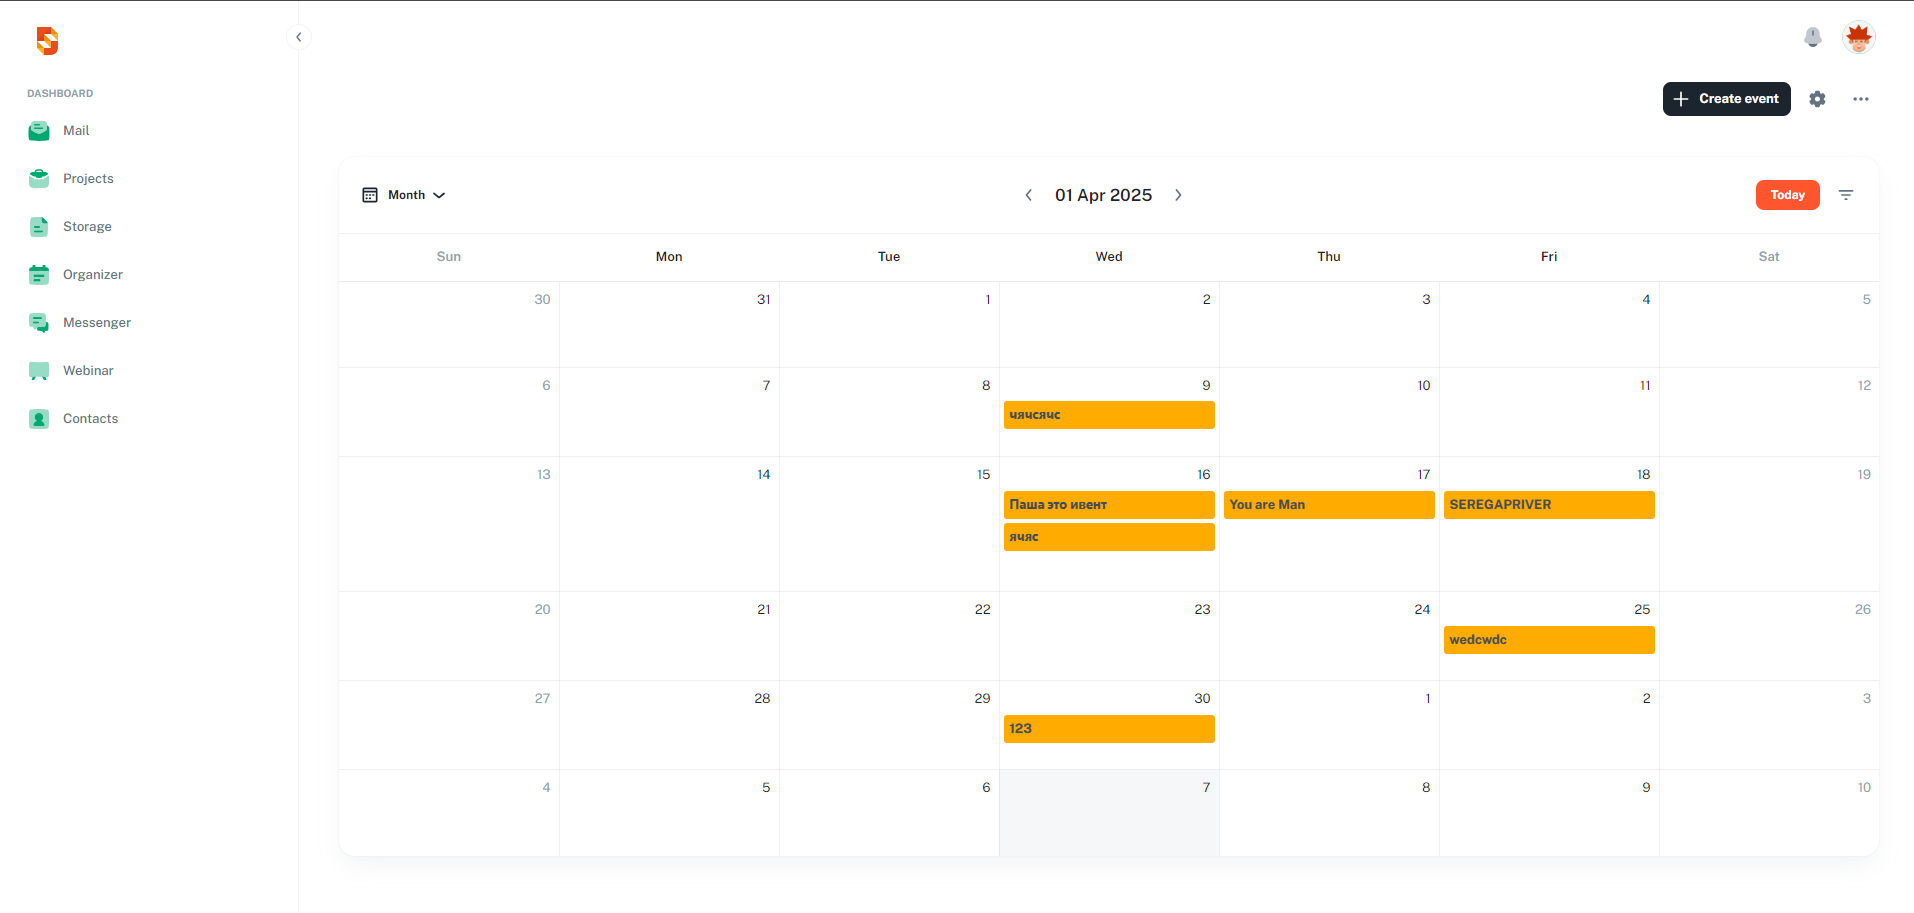
\includegraphics[width=1\linewidth]{images/календарь}
	\caption{Композиция интерфейса сервиса <<Календарь>>}
	\label{templ:image3}
\end{figure}

Композиция интерфейса создания события в сервисе <<Календарь>> представлена на рисунке \ref{templ:image3b} и состоит из:
\begin{itemize}
  \item всплывающего окна (1);
  \item кнопки для выбора категории (2);
  \item поля для ввода названия события (3);
  \item поля для ввода описания события (4);
  \item поля для ввода даты начала события и его параметров (5);
  \item поля для ввода названия видеоконференции (6);
  \item поля для выбора участников из сервиса <<Контакты>> (7);
\end{itemize}
\begin{figure}[H]
	\centering
	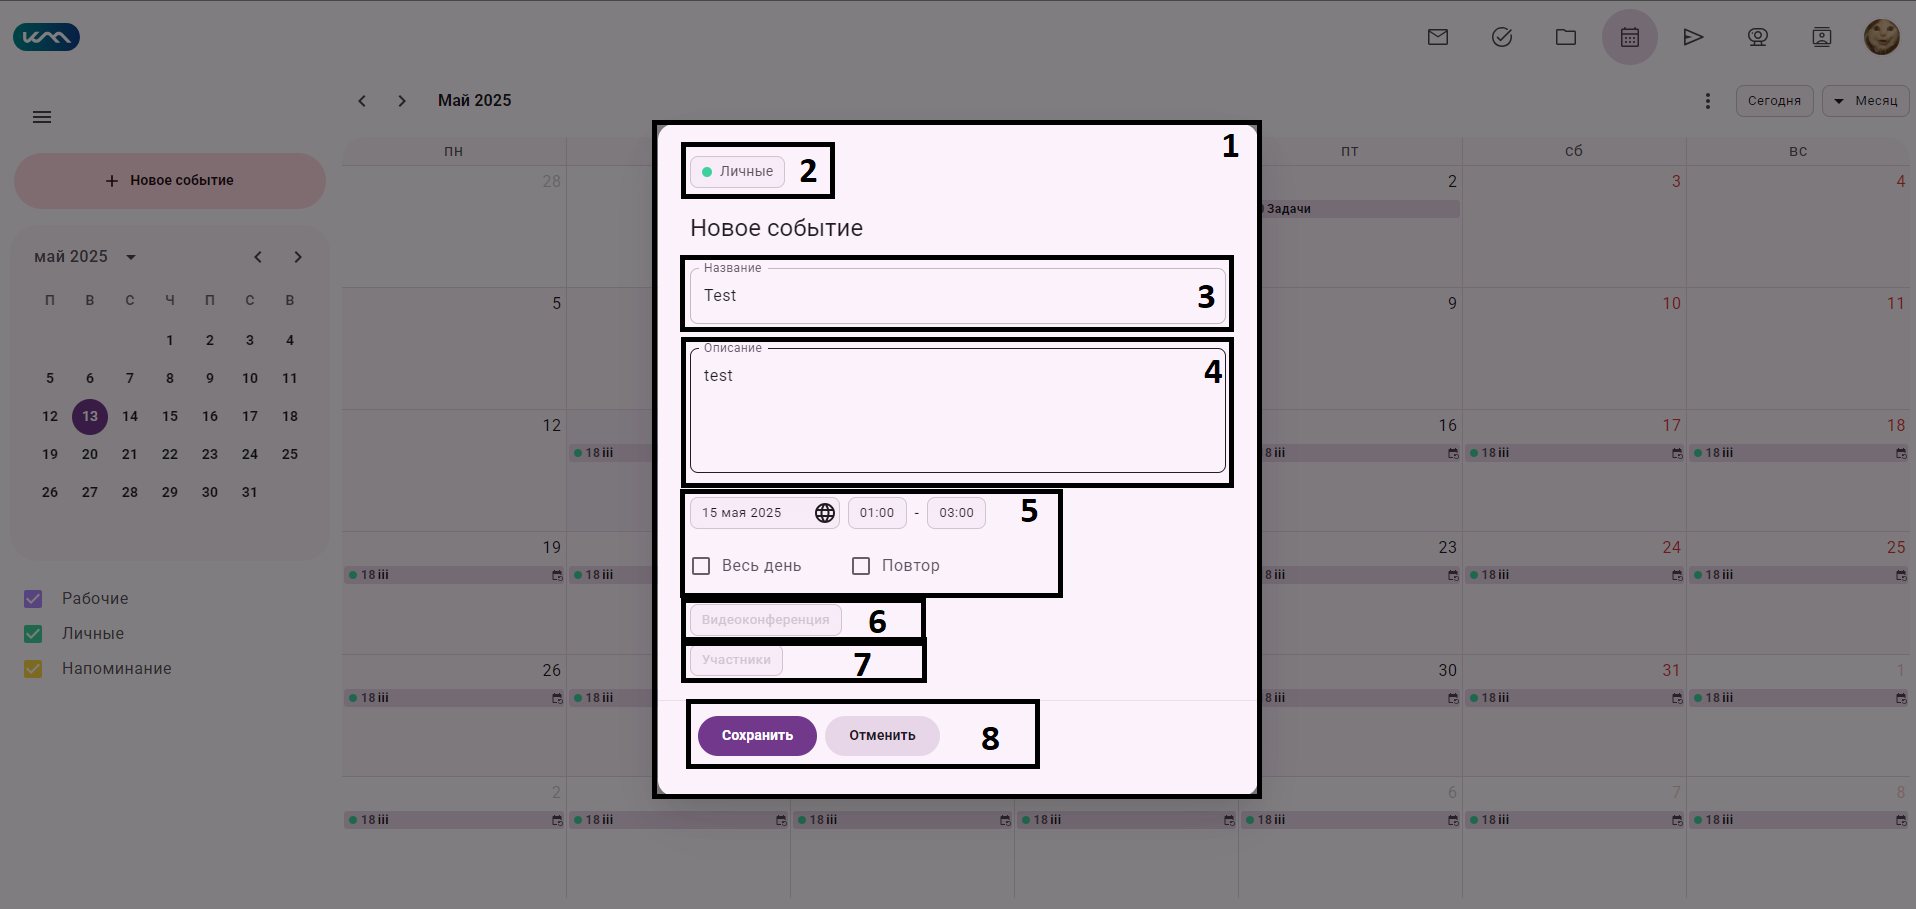
\includegraphics[width=1\linewidth]{images/календарь2}
	\caption{Композиция интерфейса создания события}
	\label{templ:image3b}
\end{figure}

Композиция интерфейса просмотра события в сервисе <<Календарь>> представлена на рисунке \ref{templ:image3c} и состоит из:
\begin{itemize}
  \item всплывающего окна (1);
  \item кнопок для редактирования, создания ссылки, удаления события (2);
  \item раздела с подробной информацией о событии (3);
  \item кнопок для подключения к ВКС, копирования события, прикрепления файла из сервиса <<Файлы>> (4);
  \item раздела с подробной информацией об участниках (5);
\end{itemize}
\begin{figure}[H]
	\centering
	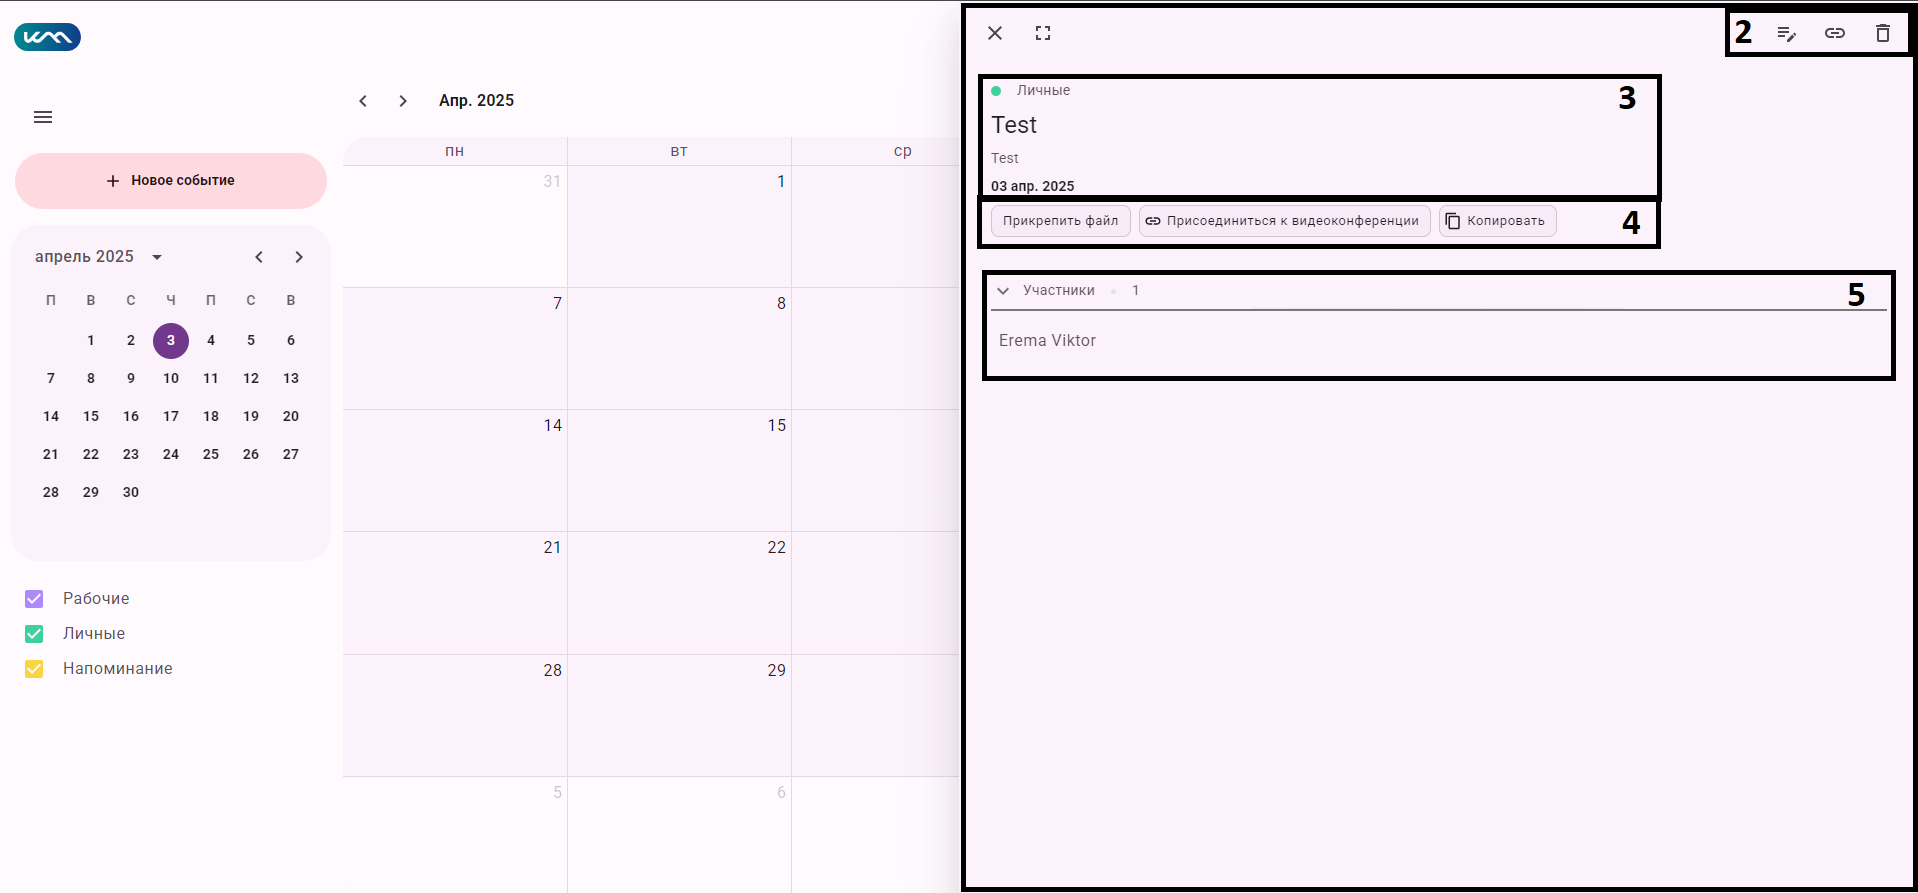
\includegraphics[width=1\linewidth]{images/календарь3}
	\caption{Композиция интерфейса просмотра события}
	\label{templ:image3c}
\end{figure}

Композиция интерфейса сервиса <<Панель управления>> представлена на рисунке \ref{templ:image4} и состоит из:
\begin{itemize}
  \item компонента навигации по сервисам (1);
  \item компонента "виджета" сервиса <<Почта>> (2);
  \item компонента "виджета" сервиса <<Проекты>> (3);
  \item компонента "виджета" сервиса <<Файлы>> (4);
  \item компонента "виджета" сервиса <<Календарь>> (5);
  \item компонента "виджета" сервиса <<Разговоры>> (6);
  \item компонента "виджета" сервиса <<Видеоконференцсвязь>> (7);
  \item компонента "виджета" сервиса <<Контакты>> (8);
\end{itemize}
\begin{figure}[H]
	\centering
	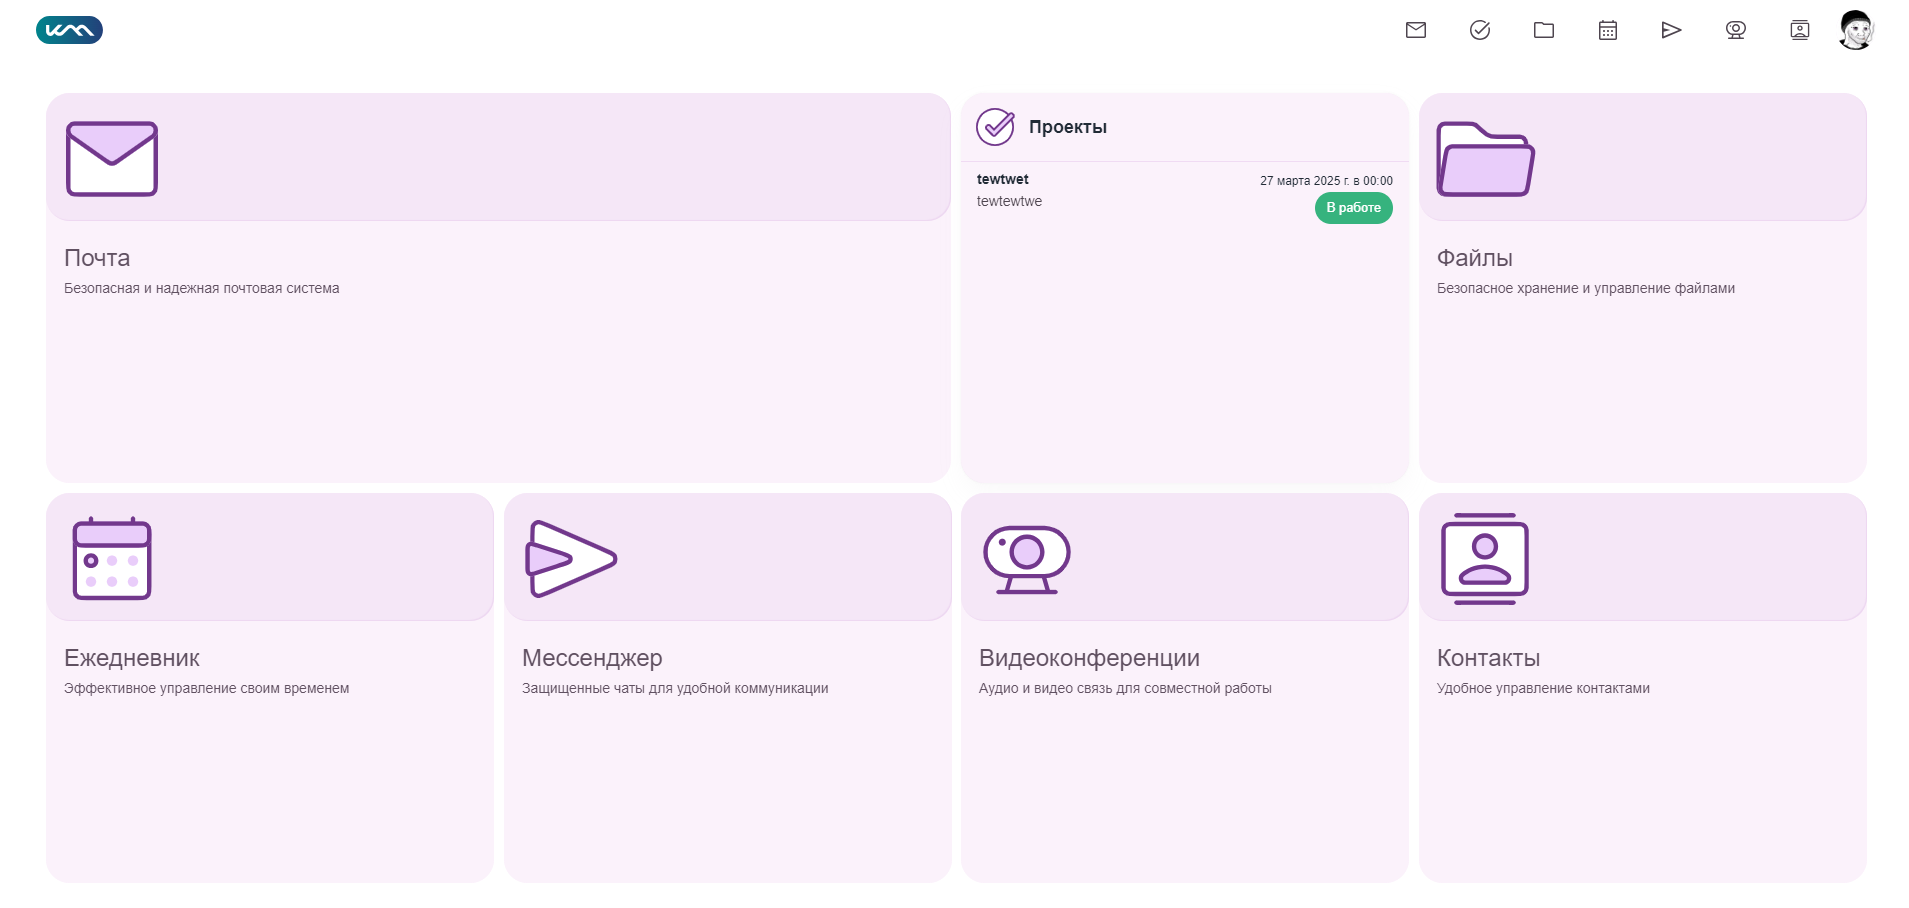
\includegraphics[width=1\linewidth]{images/дашборд}
	\caption{Композиция интерфейса сервиса <<Панель управления>>}
	\label{templ:image4}
\end{figure}

Композиция интерфейса сервиса <<Контакты>> представлена на рисунке \ref{templ:image5} и состоит из:
\begin{itemize}
  \item компонента навигации по сервисам (1);
  \item кнопки для создания контакта (2);
  \item списка папок (3);
  \item окна для работы с контактами (4);
  \item компонента пагинации (5);
\end{itemize}
\begin{figure}[H]
	\centering
	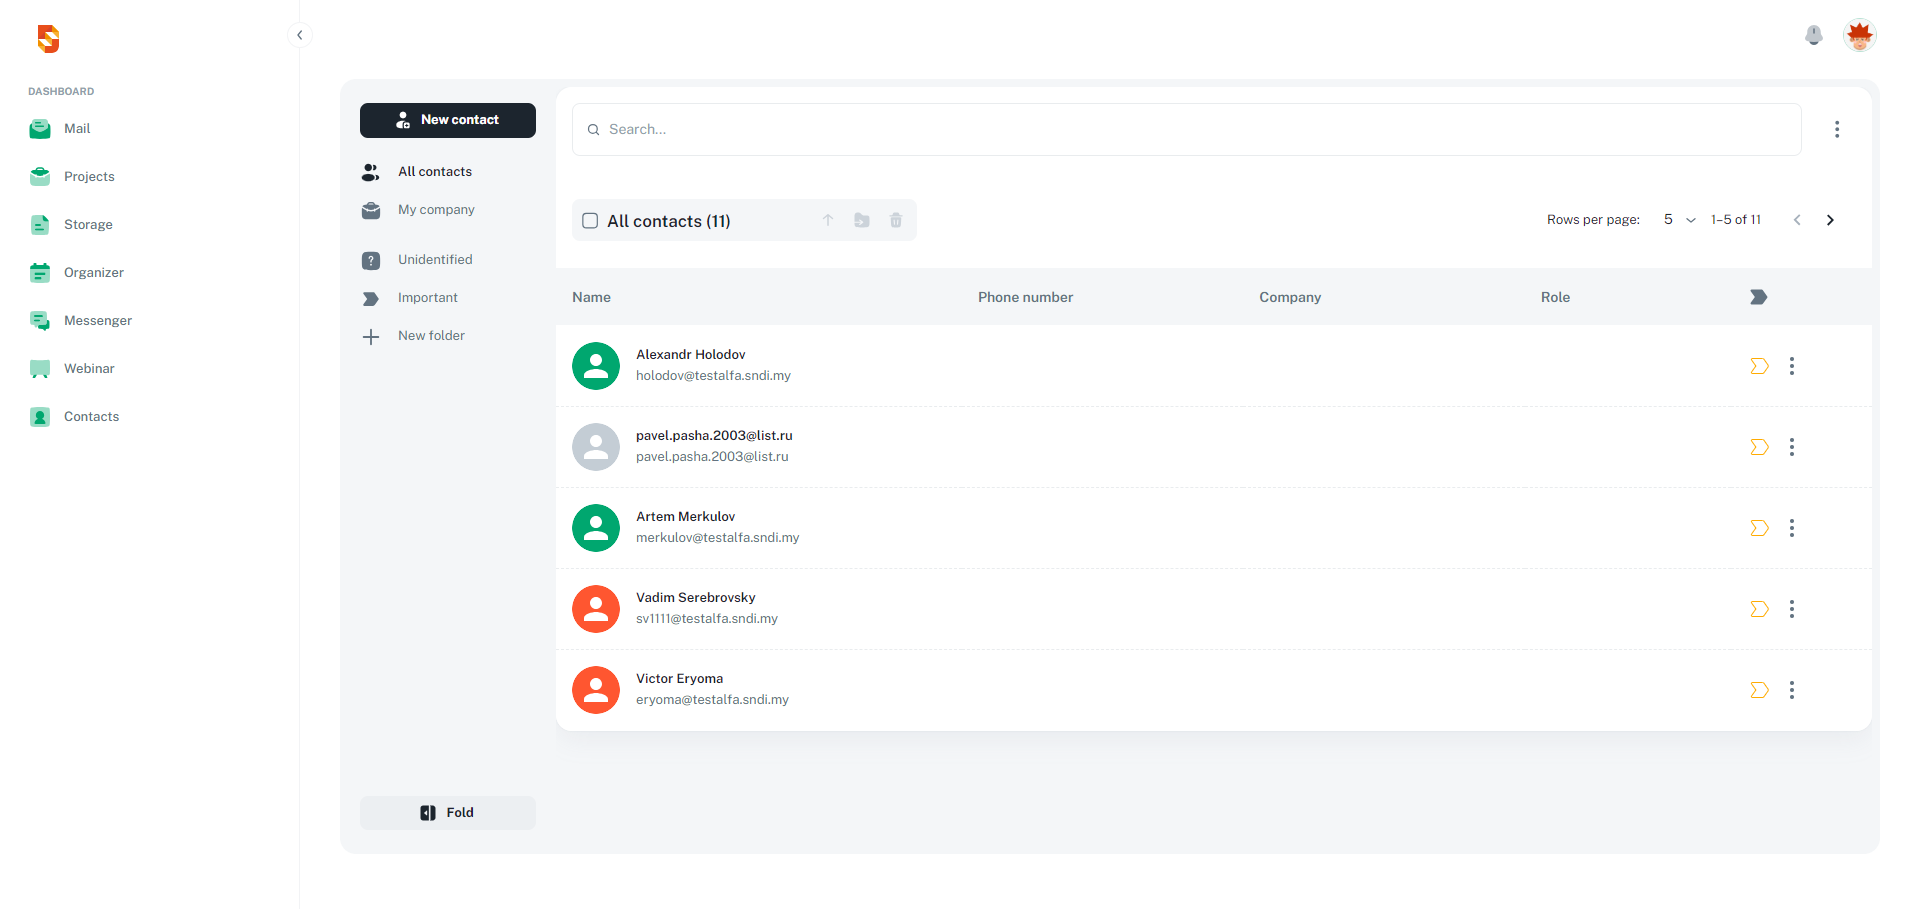
\includegraphics[width=1\linewidth]{images/контакты}
	\caption{Композиция интерфейса сервиса <<Контакты>>}
	\label{templ:image5}
\end{figure}

Композиция интерфейса создания контакта в сервисе <<Контакты>> представлена на рисунке \ref{templ:image5b} и состоит из:
\begin{itemize}
  \item всплывающего окна (1);
  \item поля для ввода имени (2);
  \item поля для ввода фамилии (3);
  \item поля для ввода даты рождения (4);
  \item поля для ввода компании (5);
  \item поля для ввода должности (6);
  \item поля для ввода почты (7);
  \item поля для ввода телефона (8);
  \item кнопок действий (9);
\end{itemize}
\begin{figure}[H]
	\centering
	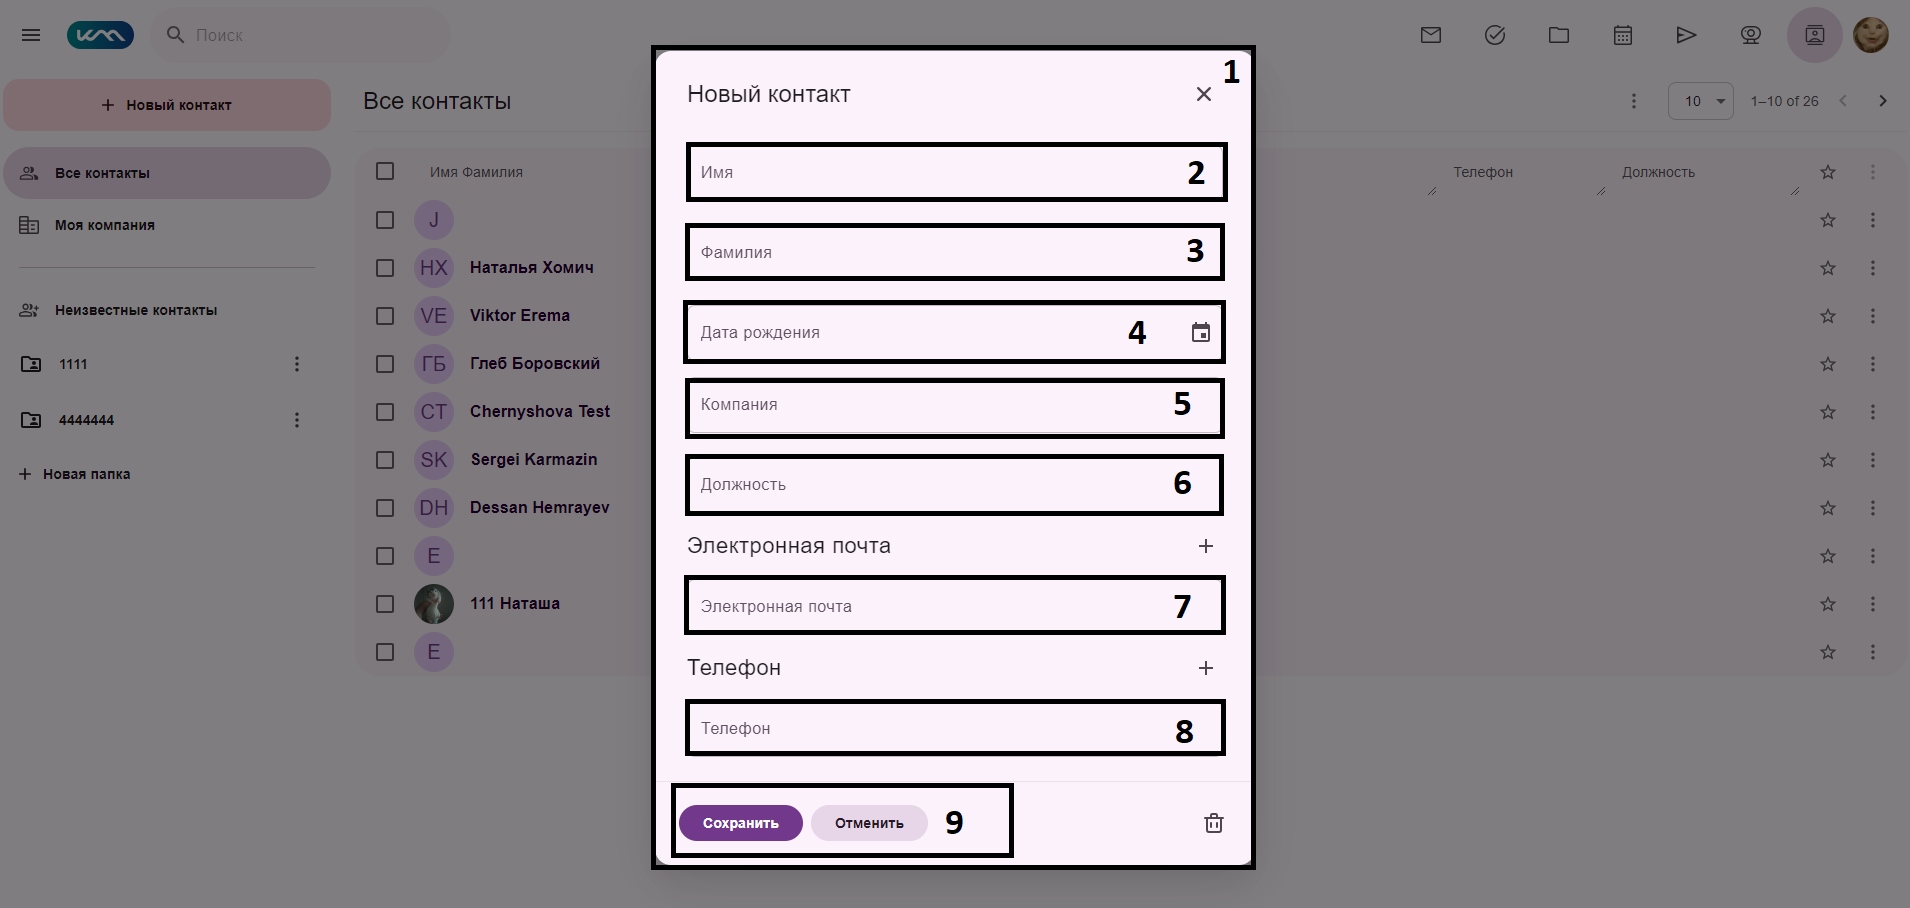
\includegraphics[width=1\linewidth]{images/контакты2}
	\caption{Композиция интерфейса создания контакта}
	\label{templ:image5b}
\end{figure}

Композиция интерфейса просмотра контакта в сервисе <<Контакты>> представлена на рисунке \ref{templ:image5b} и состоит из:
\begin{itemize}
  \item окна с информацией о контакте (1);
  \item кнопок для скачивания, редактирования, удаления и отправки контакта (2);
  \item кнопки для написания письма этому человеку в сервисе <<Почта>> (3);
  \item окна с подробной информацией о контакте (4);
\end{itemize}
\begin{figure}[H]
	\centering
	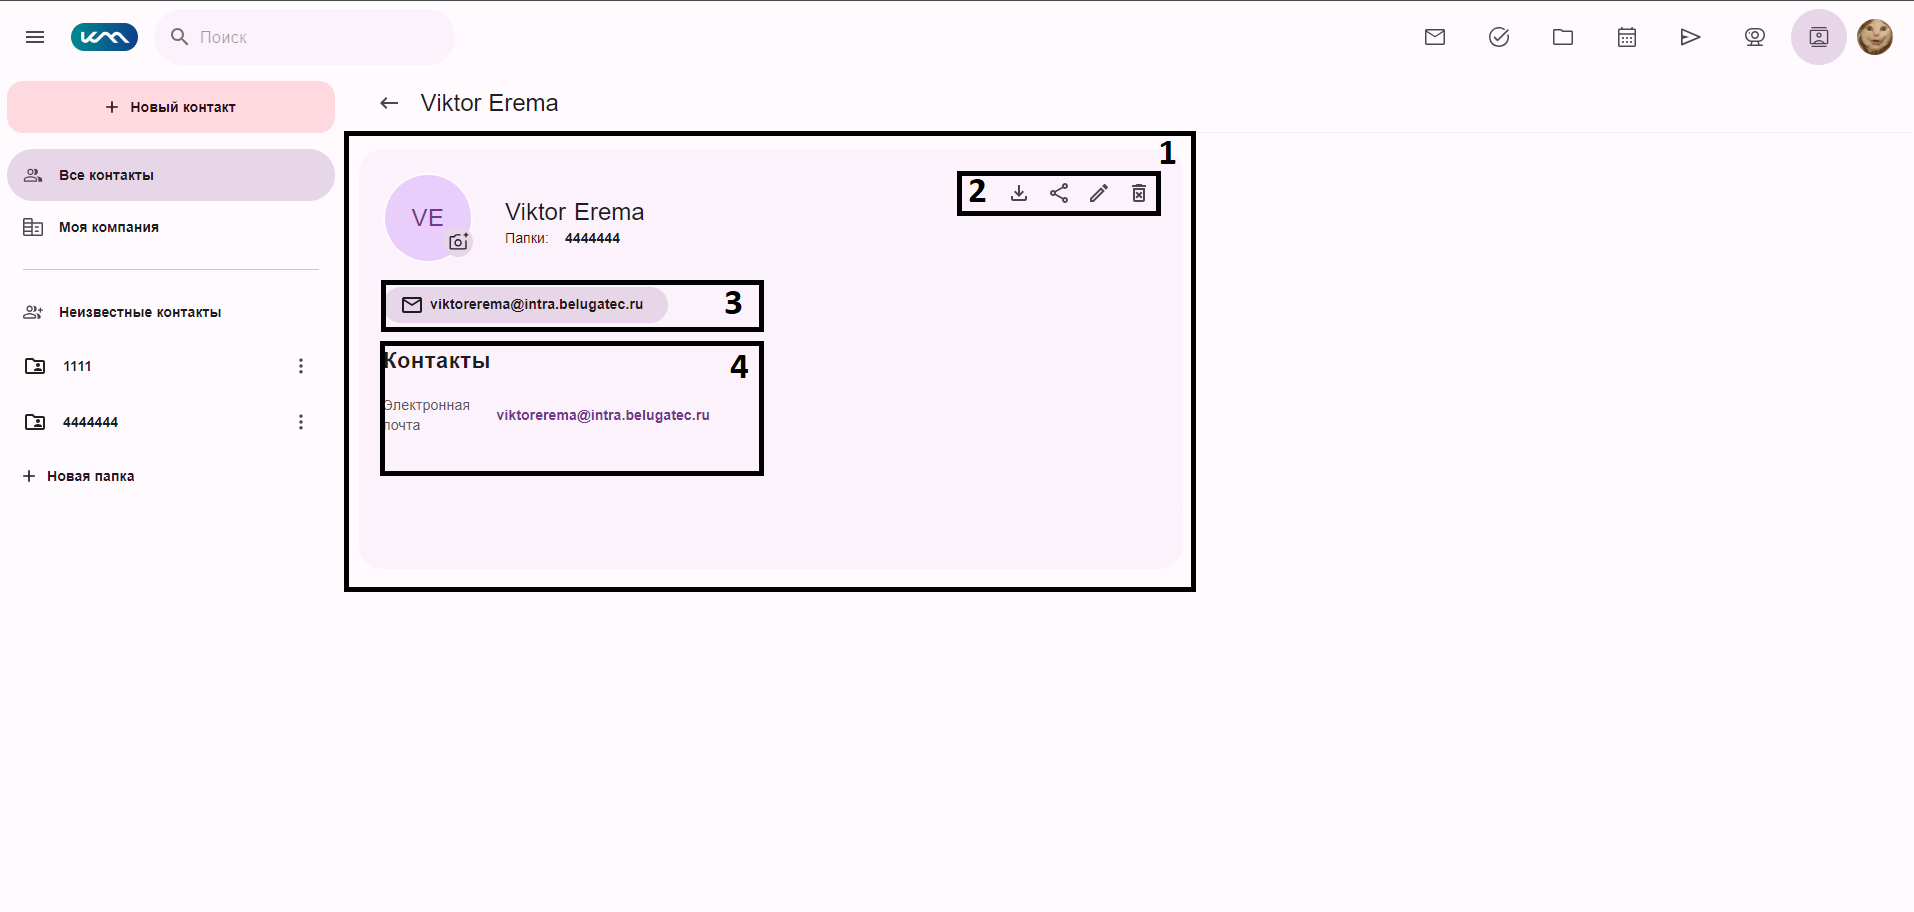
\includegraphics[width=1\linewidth]{images/контакты3}
	\caption{Композиция интерфейса просмотра контакта}
	\label{templ:image5b}
\end{figure}

Композиция интерфейса создания папки в сервисе <<Контакты>> представлена на рисунке \ref{templ:image5c} и состоит из:
\begin{itemize}
  \item всплывающего окна (1);
  \item поля для ввода названия папки (2);
  \item кнопок действий (3);
\end{itemize}
\begin{figure}[H]
	\centering
	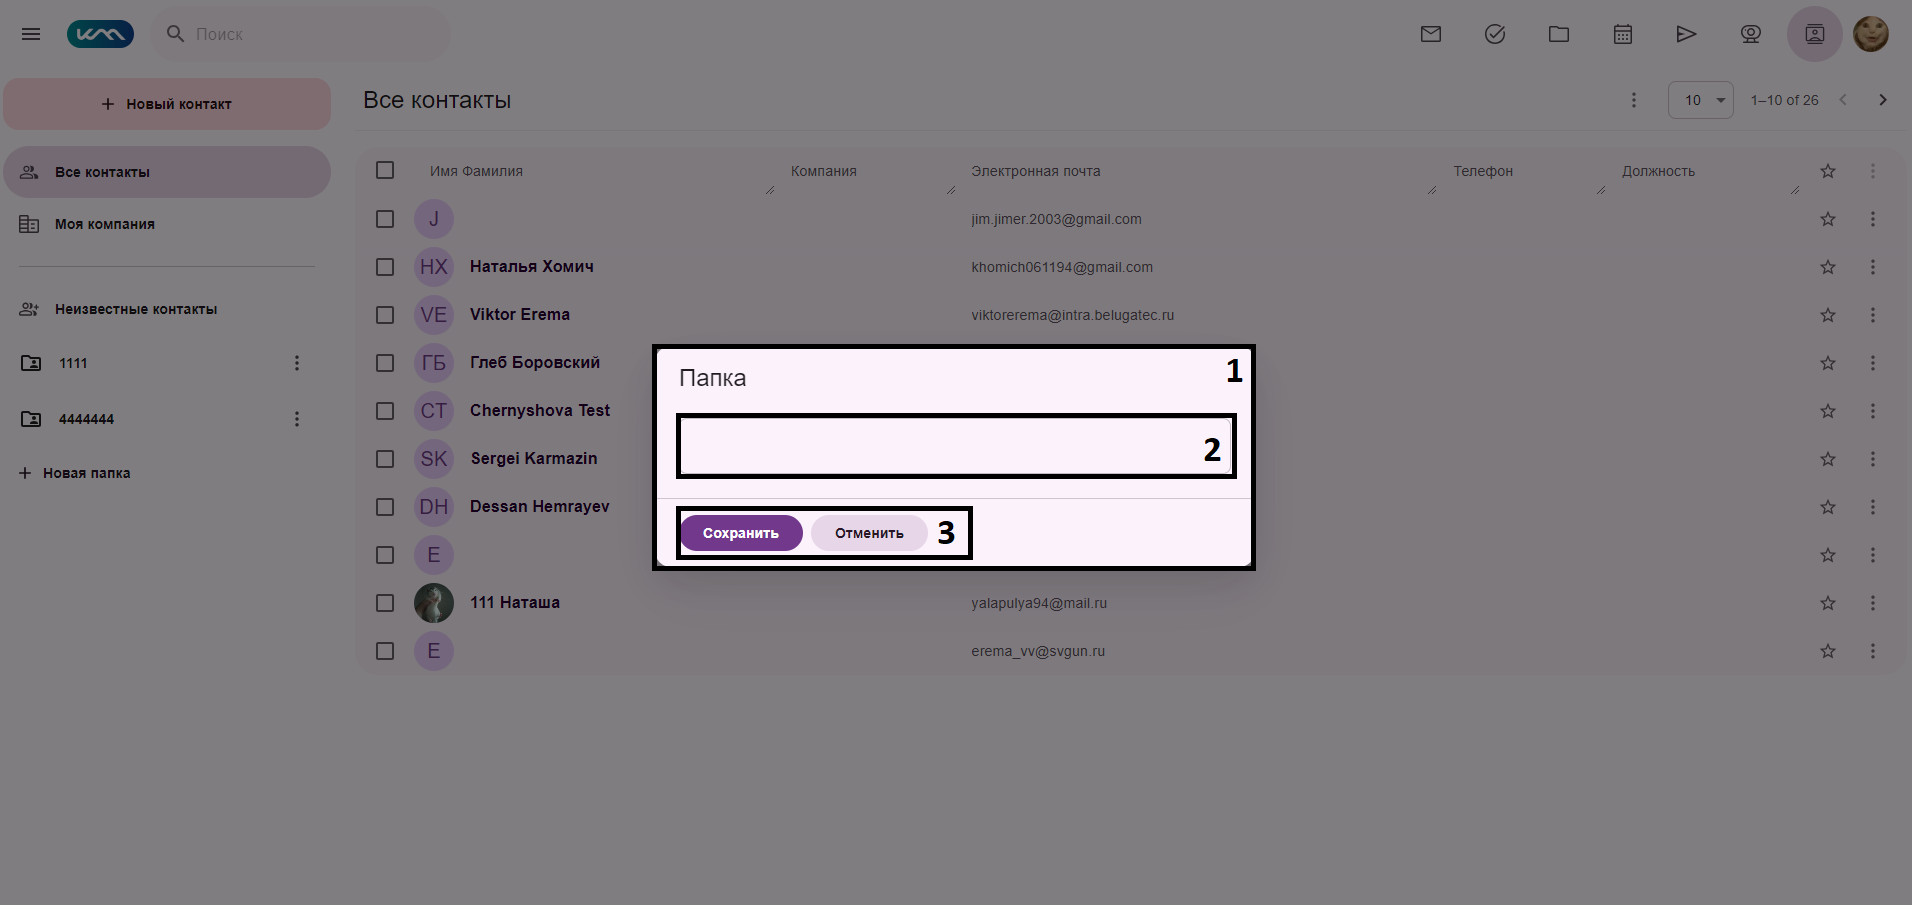
\includegraphics[width=1\linewidth]{images/контакты4}
	\caption{Композиция интерфейса создания папки}
	\label{templ:image5c}
\end{figure}

Композиция интерфейса сервиса <<Настройки>> представлена на рисунке \ref{templ:image6} и состоит из:
\begin{itemize}
  \item компонента навигации по сервисам (1);
  \item компонента навигации по разделам (2);
  \item кнопки для выхода из учётной записи (3);
  \item раздела смены темы (4);
  \item раздела смены цветовой палитры (5);
  \item раздела редактирования подписи электронной почты (6);
\end{itemize}
\begin{figure}[H]
	\centering
	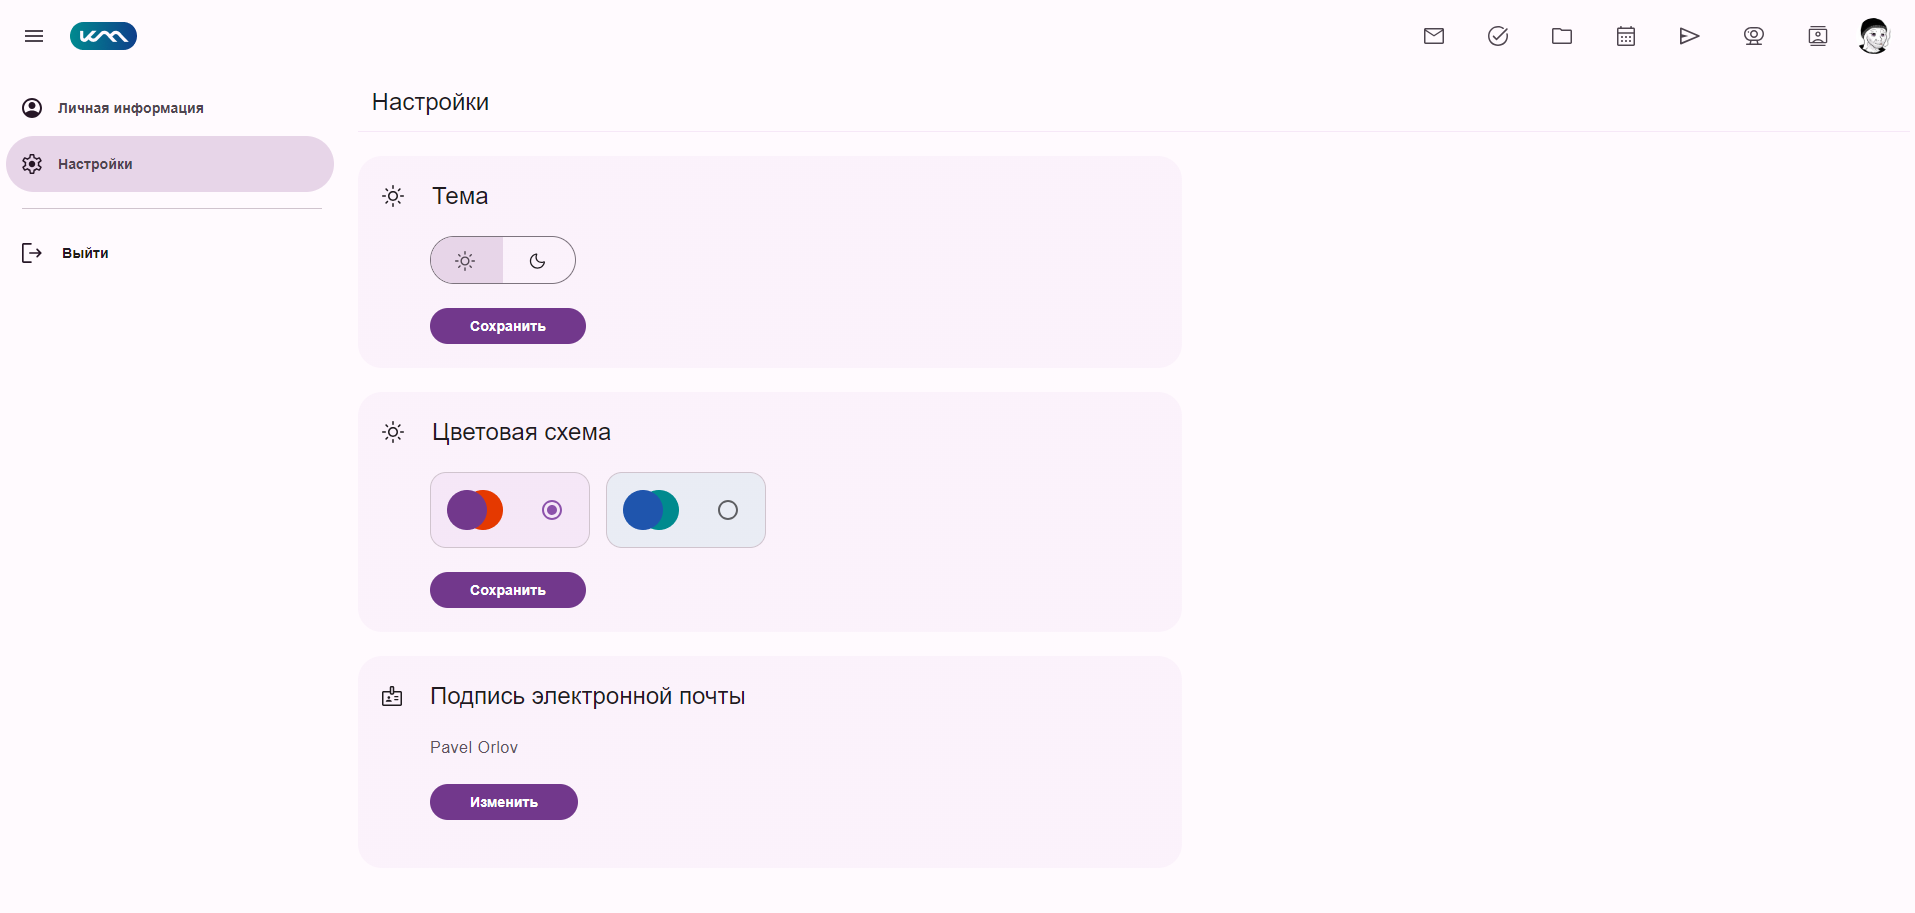
\includegraphics[width=1\linewidth]{images/настройки}
	\caption{Композиция интерфейса сервиса <<Настройки>>}
	\label{templ:image6}
\end{figure}

Композиция интерфейса изменения цифровой подписи в сервисе <<Настройки>> представлена на рисунке \ref{templ:image6b} и состоит из:
\begin{itemize}
  \item всплывающего окна (1);
  \item поля для ввода цифровой подписи (2);
  \item кнопок действий (3);
\end{itemize}
\begin{figure}[H]
	\centering
	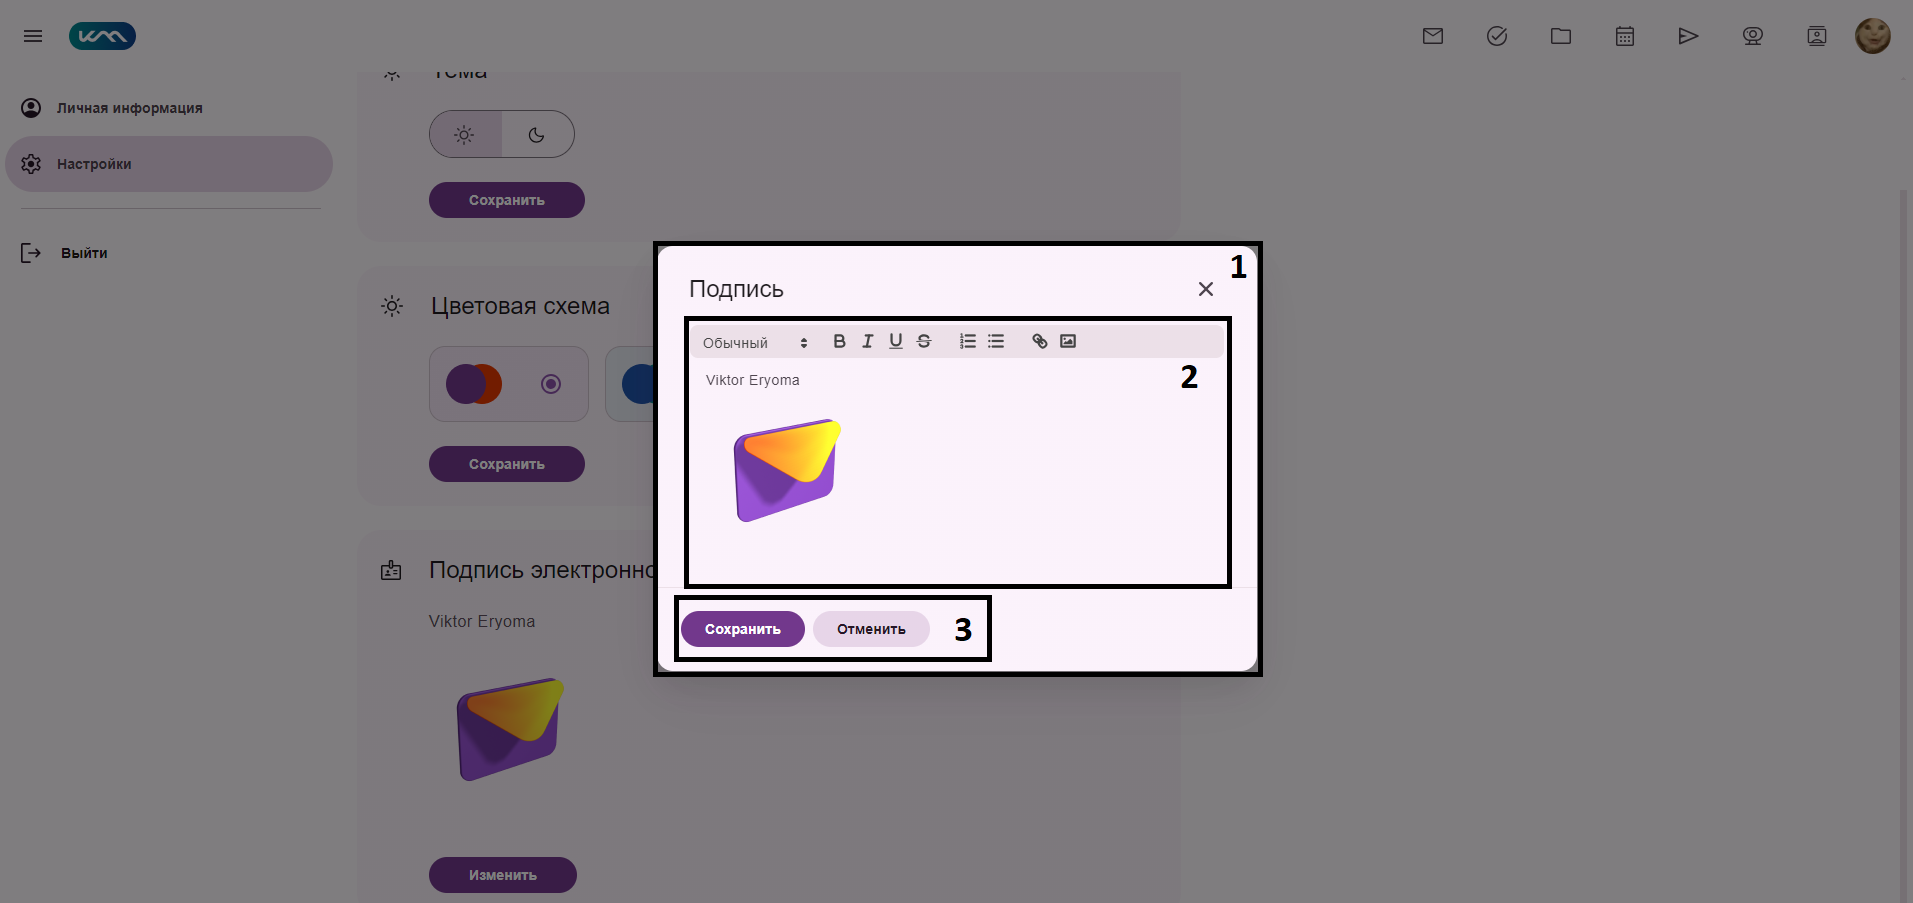
\includegraphics[width=1\linewidth]{images/настройки2}
	\caption{Композиция интерфейса изменения цифровой подписи}
	\label{templ:image6b}
\end{figure}

Композиция интерфейса сервиса <<Проекты>> представлена на рисунке \ref{templ:image7} и состоит из:
\begin{itemize}
  \item компонента навигации по сервисам (1);
  \item кнопки для создания раздела (2);
  \item компонента навигации по разделам (3);
  \item окна для работы с задачами (4);
  \item кнопки для создания задачи (5);
\end{itemize}
\begin{figure}[H]
	\centering
	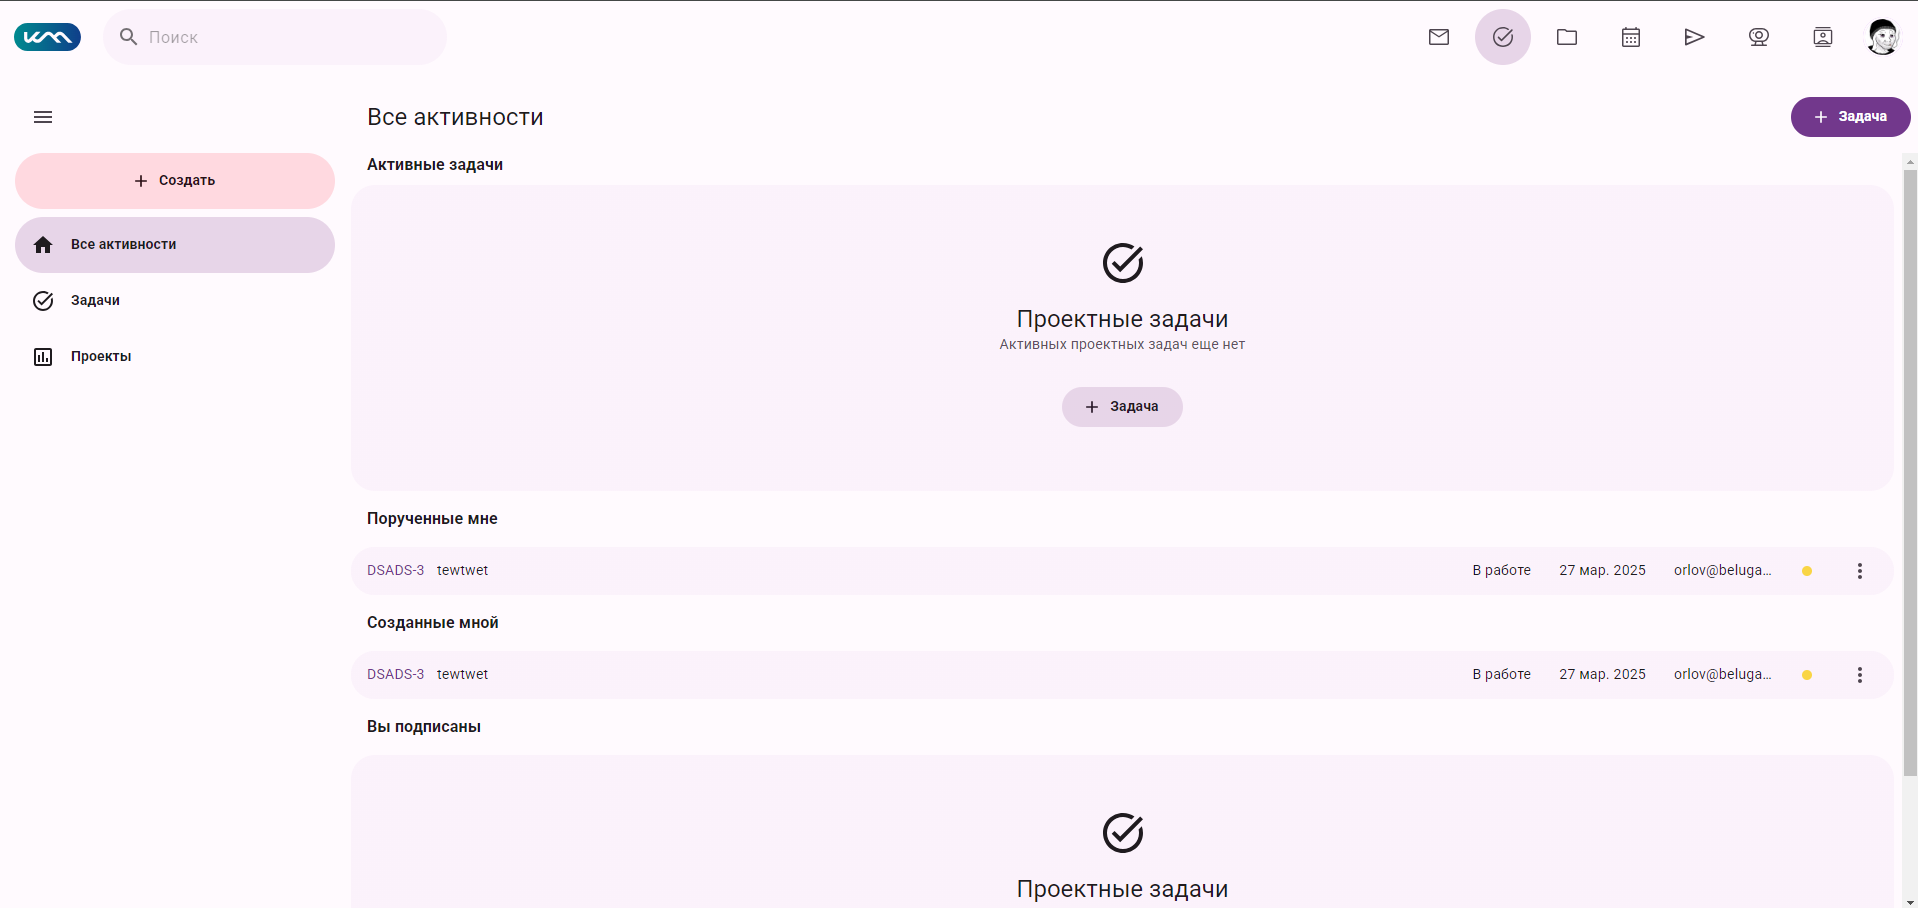
\includegraphics[width=1\linewidth]{images/проекты}
	\caption{Композиция интерфейса сервиса <<Проекты>>}
	\label{templ:image7}
\end{figure}

Композиция интерфейса создания проекта в сервисе <<Проекты>> представлена на рисунке \ref{templ:image7b} и состоит из:
\begin{itemize}
  \item всплывающего окна (1);
  \item поля для ввода названия проекта (2);
  \item поля для ввода описания проекта (3);
  \item кнопок действий (4);
\end{itemize}
\begin{figure}[H]
	\centering
	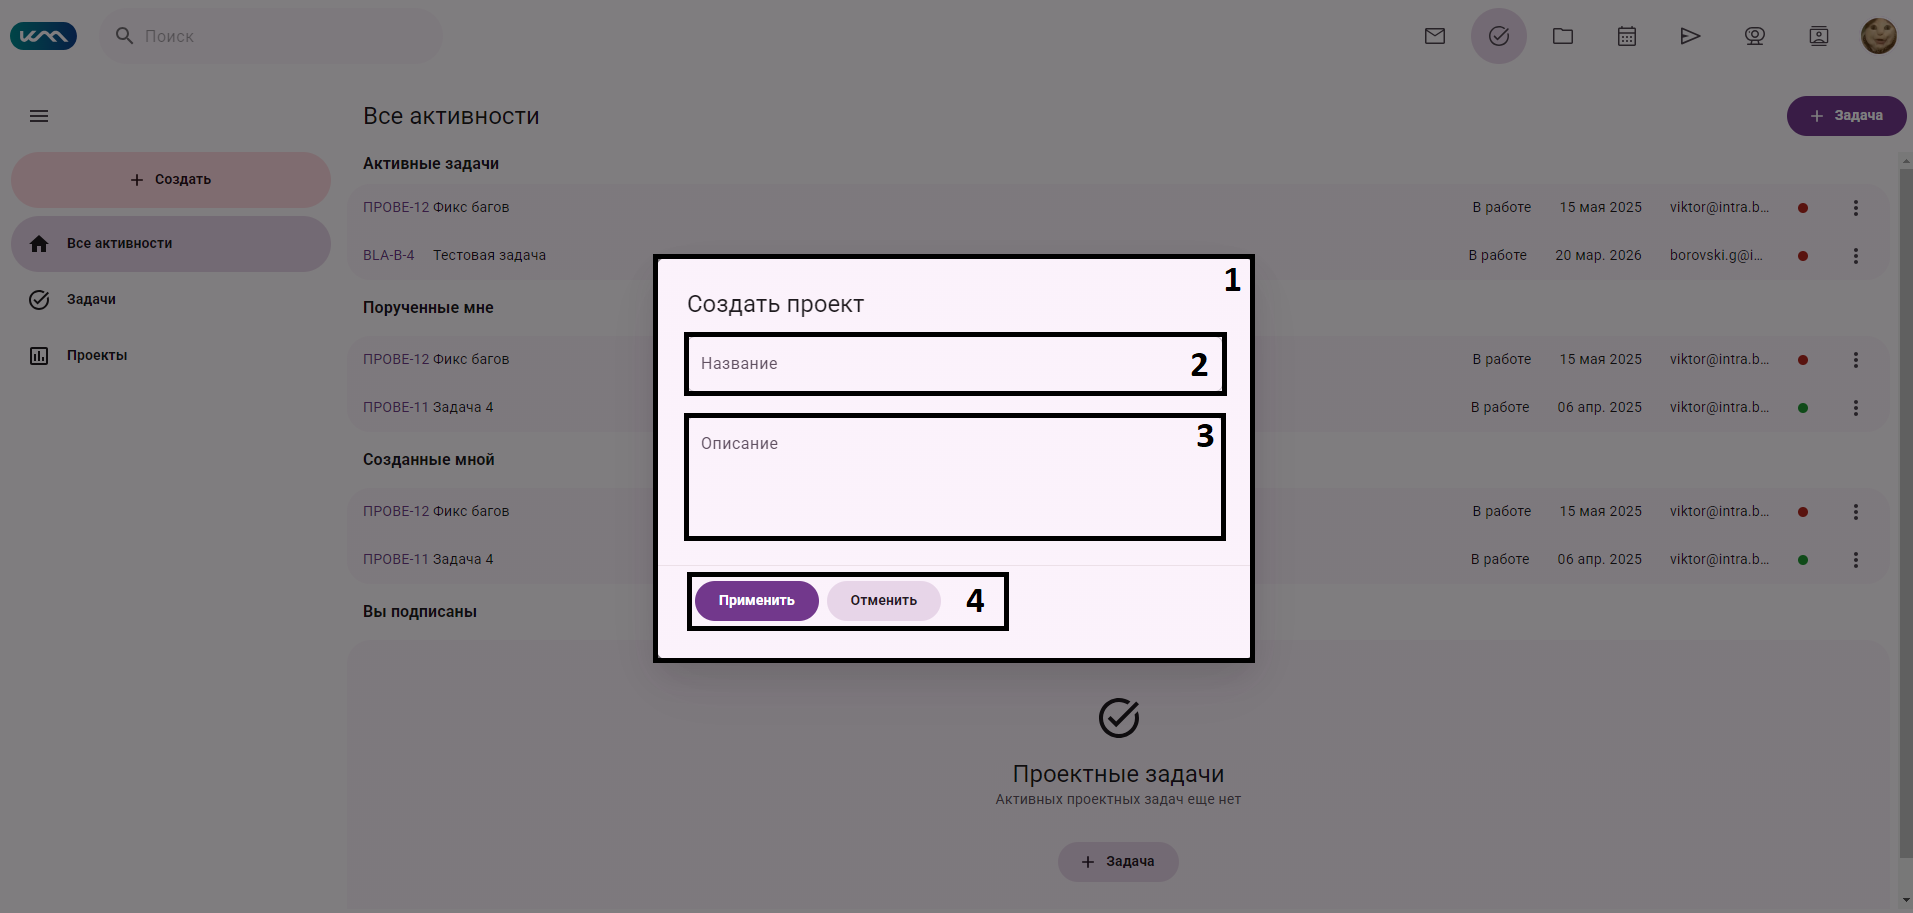
\includegraphics[width=1\linewidth]{images/проекты2}
	\caption{Композиция интерфейса создания проекта}
	\label{templ:image7b}
\end{figure}

Композиция интерфейса создания задачи в сервисе <<Проекты>> представлена на рисунке \ref{templ:image7c} и состоит из:
\begin{itemize}
  \item всплывающего окна (1);
  \item кнопки для выбора проекта (2);
  \item поля для ввода названия задачи (3);
  \item поля для ввода описания задачи (4);
  \item кнопок для выбора даты начала/конца задачи, приоритета, исполнителя (5);
  \item кнопок действий (6);
\end{itemize}
\begin{figure}[H]
	\centering
	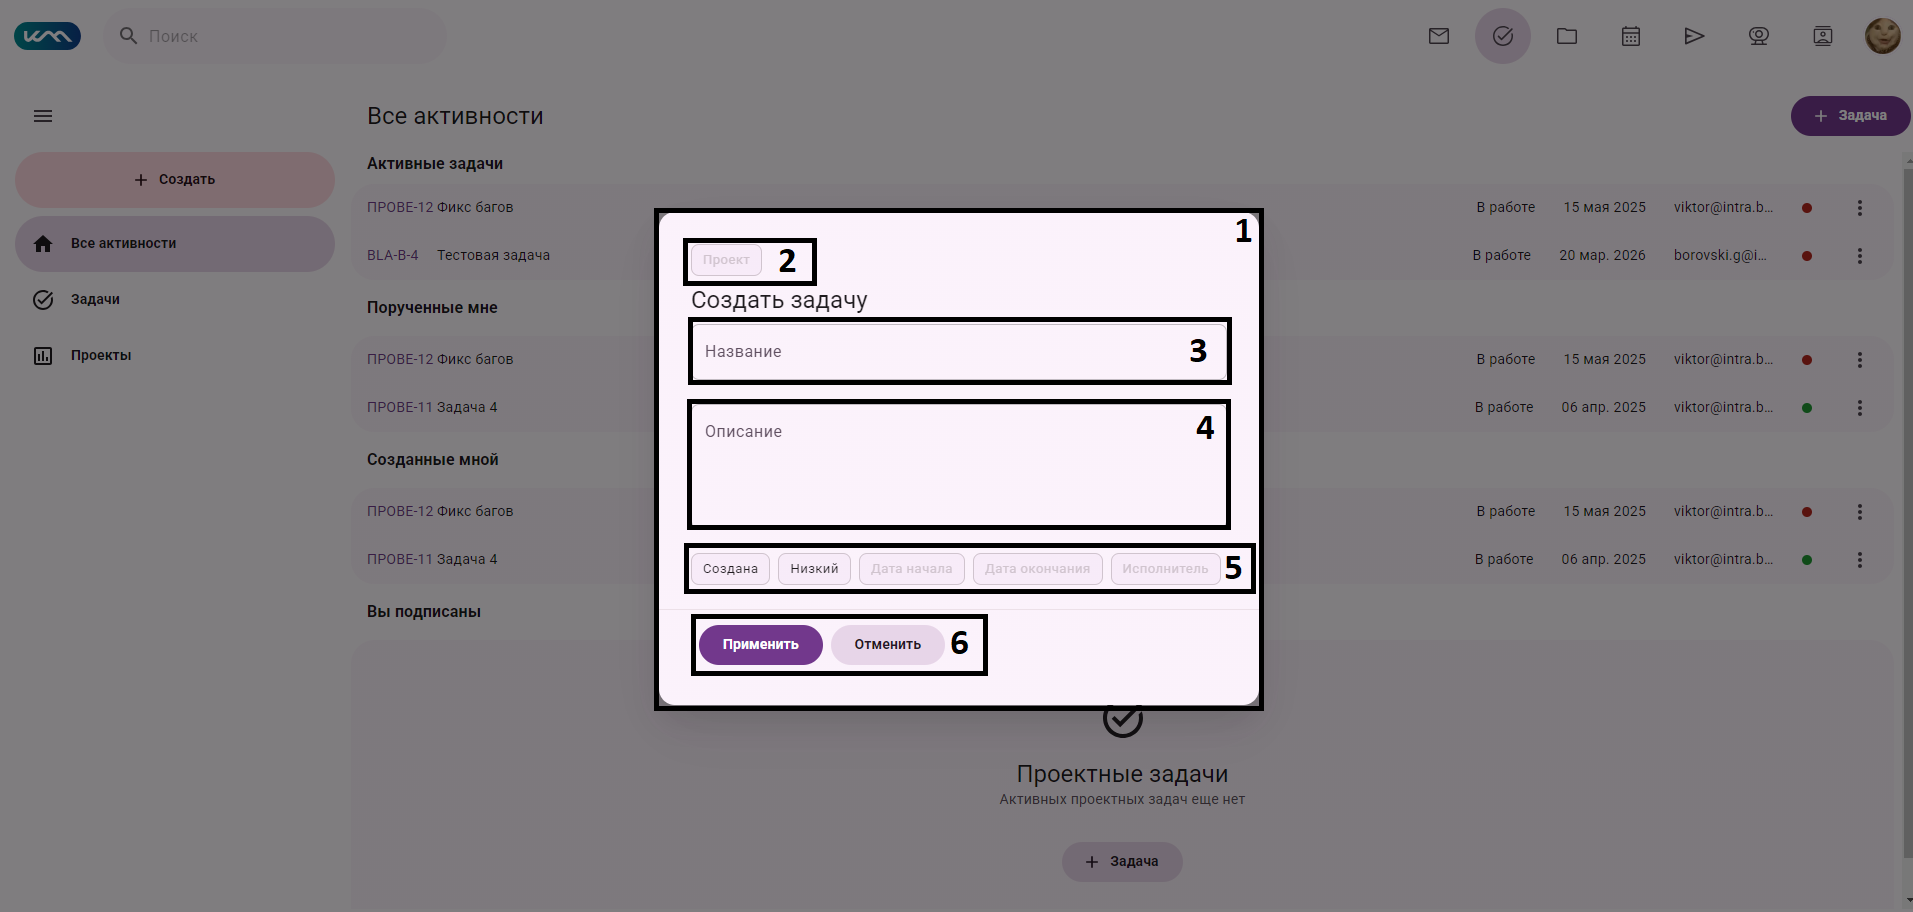
\includegraphics[width=1\linewidth]{images/проекты3}
	\caption{Композиция интерфейса создания задачи}
	\label{templ:image7c}
\end{figure}

Композиция интерфейса просмотра задачи в сервисе <<Проекты>> представлена на рисунке \ref{templ:image7d} и состоит из:
\begin{itemize}
  \item всплывающего окна (1);
  \item кнопок для отслеживания, удаления и архивирования задачи (2);
  \item подробной информации о задаче (3);
  \item кнопок для прикрепления файлов/ссылок, добавление подзадачи (4);
  \item раздела с комментариями (5);
  \item поля для ввода комментария (6);
  \item кнопки для отправки комментария (7);
\end{itemize}
\begin{figure}[H]
	\centering
	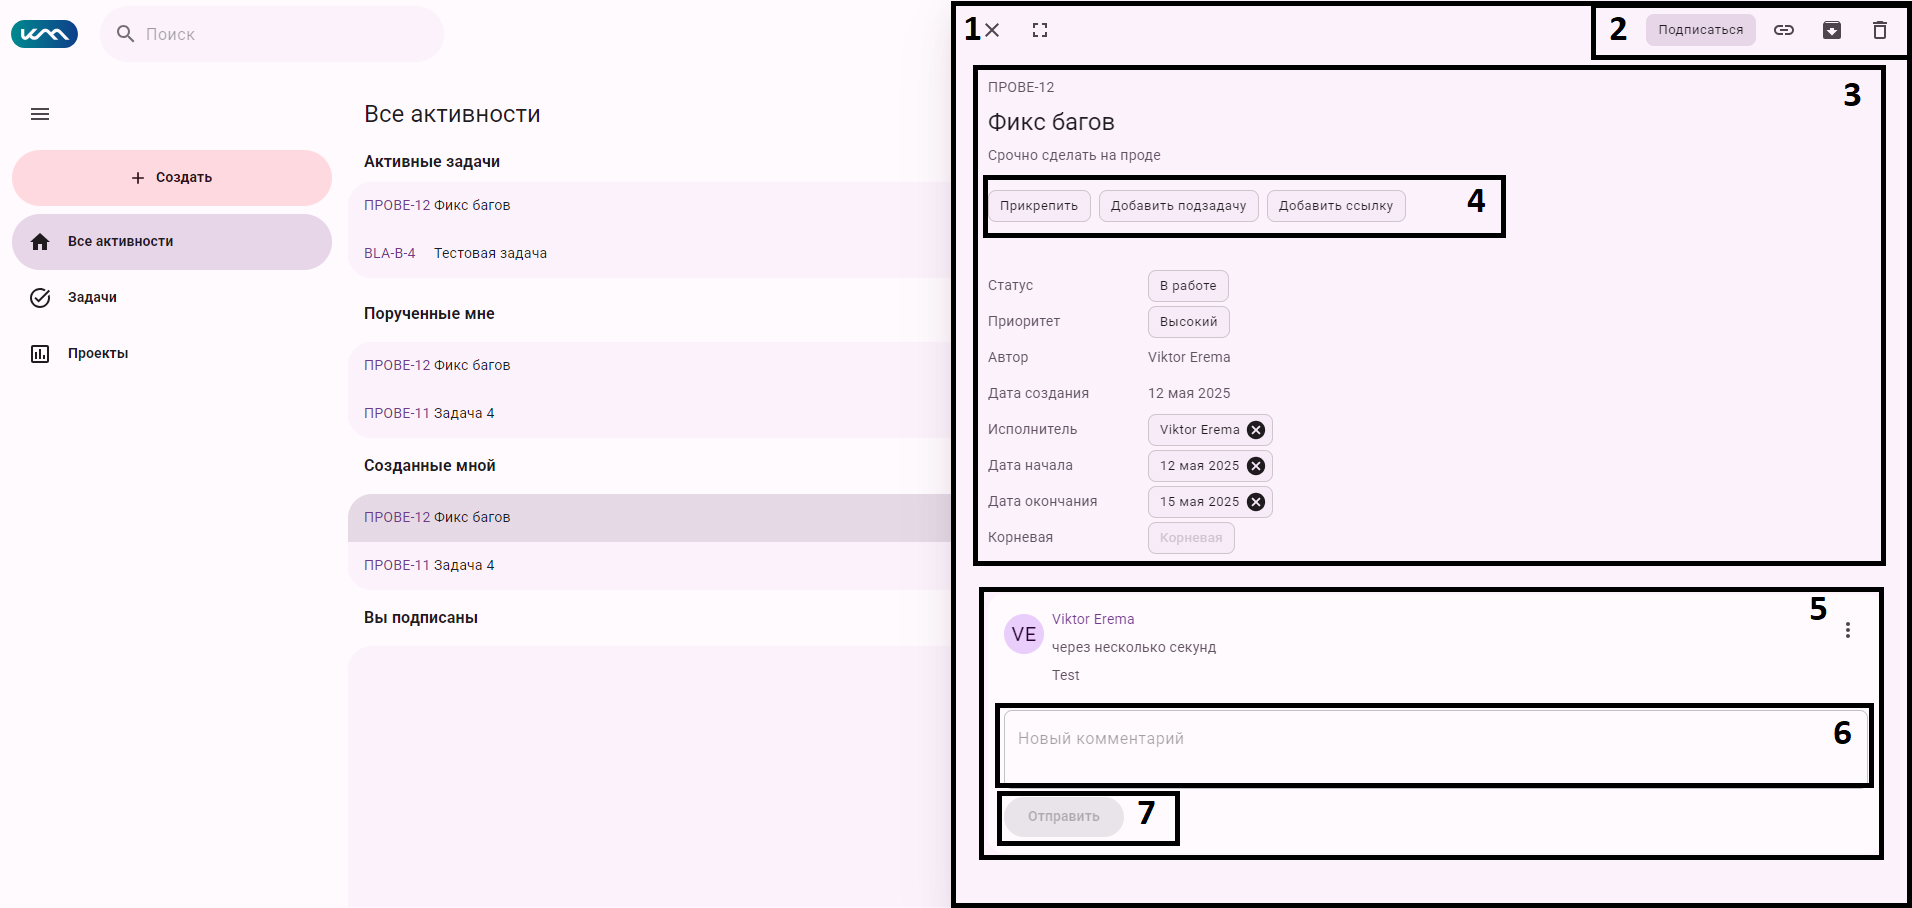
\includegraphics[width=1\linewidth]{images/проекты4}
	\caption{Композиция интерфейса просмотра задачи}
	\label{templ:image7d}
\end{figure}

Композиция интерфейса сервиса <<Разговоры>> представлена на рисунке \ref{templ:image8} и состоит из:
\begin{itemize}
  \item компонента навигации по сервисам (1);
  \item кнопки для создания комнаты (2);
  \item списка комнат (3);
  \item кнопки для создания диалога (4);
  \item кнопки для создания канала (5);
  \item окна для работы с комнатой (6);
  \item поля для написания сообщения (7);
\end{itemize}
\begin{figure}[H]
	\centering
	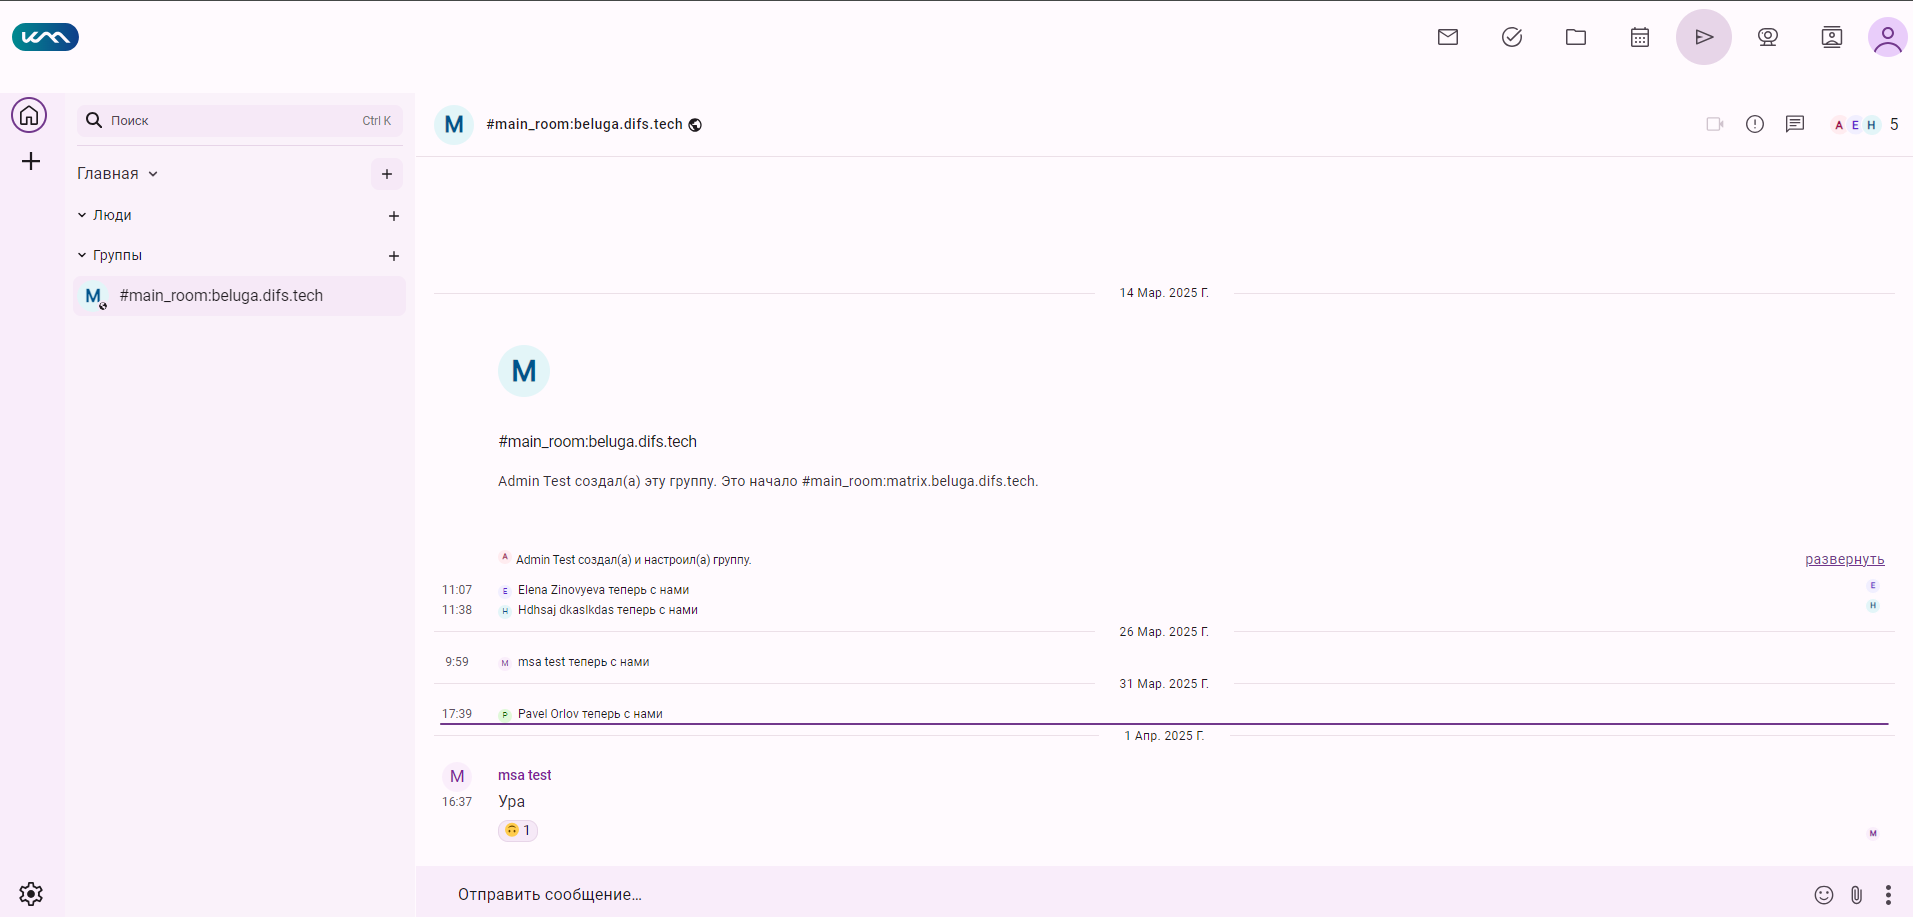
\includegraphics[width=1\linewidth]{images/разговоры}
	\caption{Композиция интерфейса сервиса <<Разговоры>>}
	\label{templ:image8}
\end{figure}

Композиция интерфейса сервиса <<Файлы>> представлена на рисунке \ref{templ:image9} и состоит из:
\begin{itemize}
  \item компонента навигации по сервисам (1);
  \item кнопки для создания папки/загрузки файла в текущую папку (2);
  \item списка папок (3);
  \item окна для работы с файлами (4);
  \item кнопки для перехода в настройки сервиса (5);
\end{itemize}
\begin{figure}[H]
	\centering
	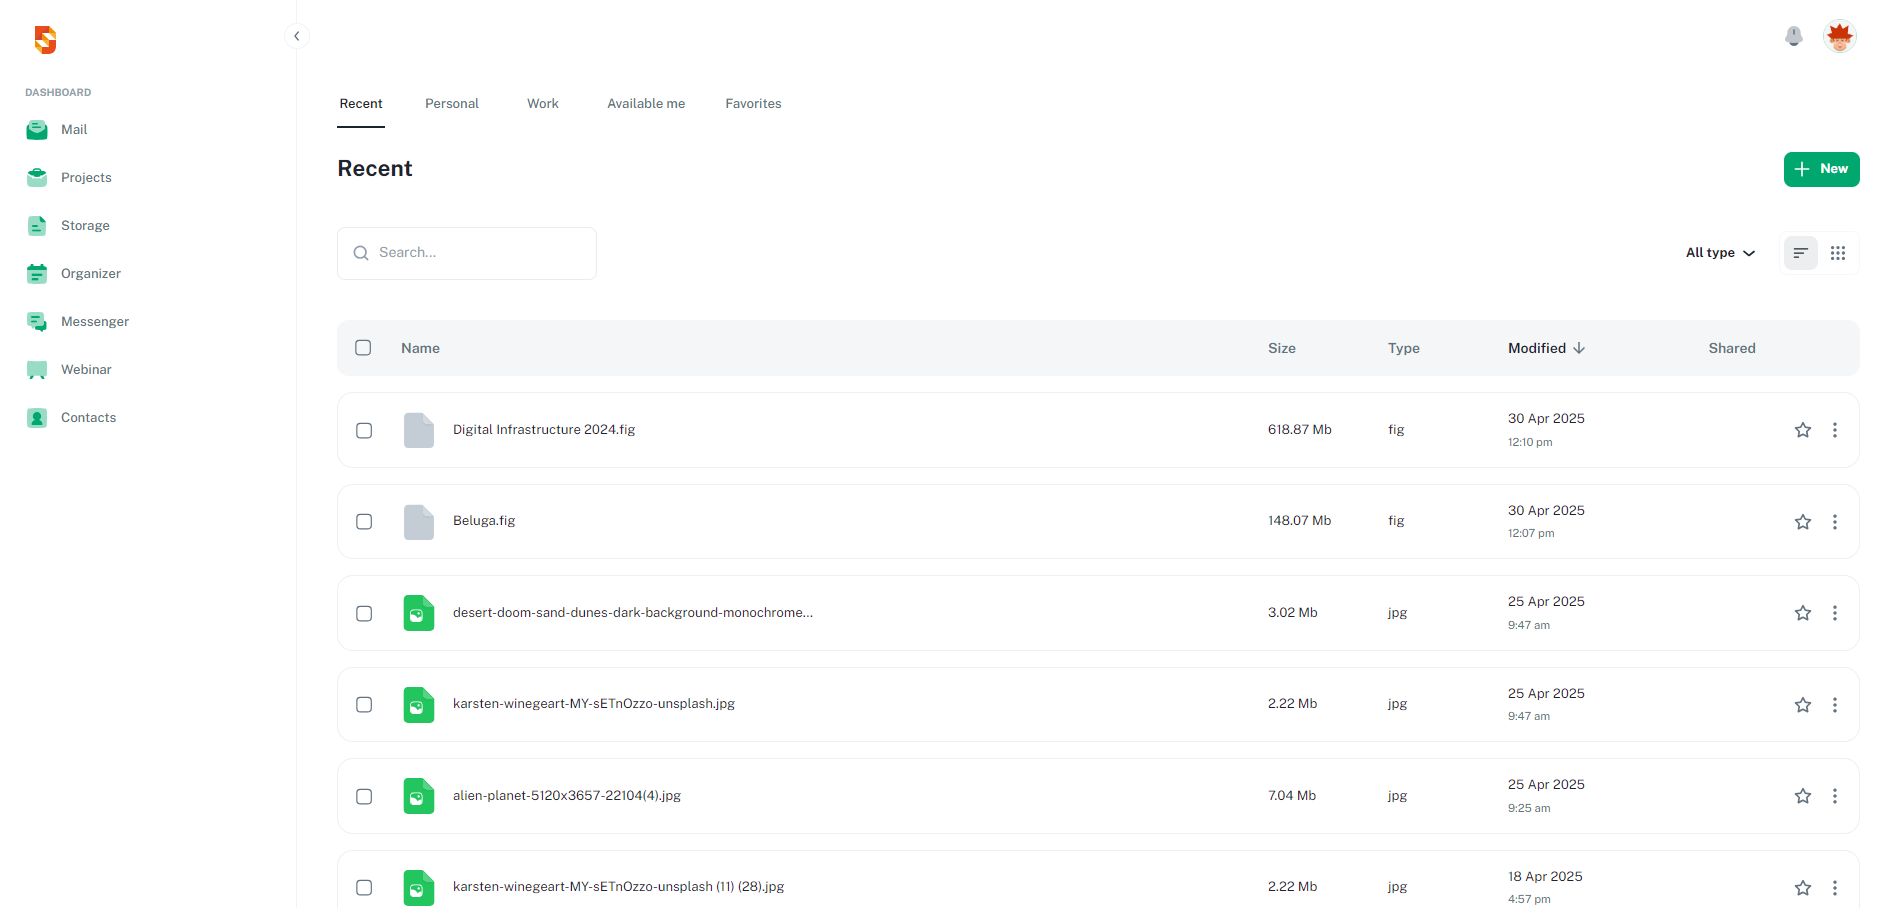
\includegraphics[width=1\linewidth]{images/файлы}
	\caption{Композиция интерфейса сервиса <<Файлы>>}
	\label{templ:image9}
\end{figure}

Композиция интерфейса создания файла в сервисе <<Файлы>> представлена на рисунке \ref{templ:image9b} и состоит из:
\begin{itemize}
  \item всплывающего окна (1);
  \item поля для ввода названия файла (2);
  \item кнопок действий (3);
\end{itemize}
\begin{figure}[H]
	\centering
	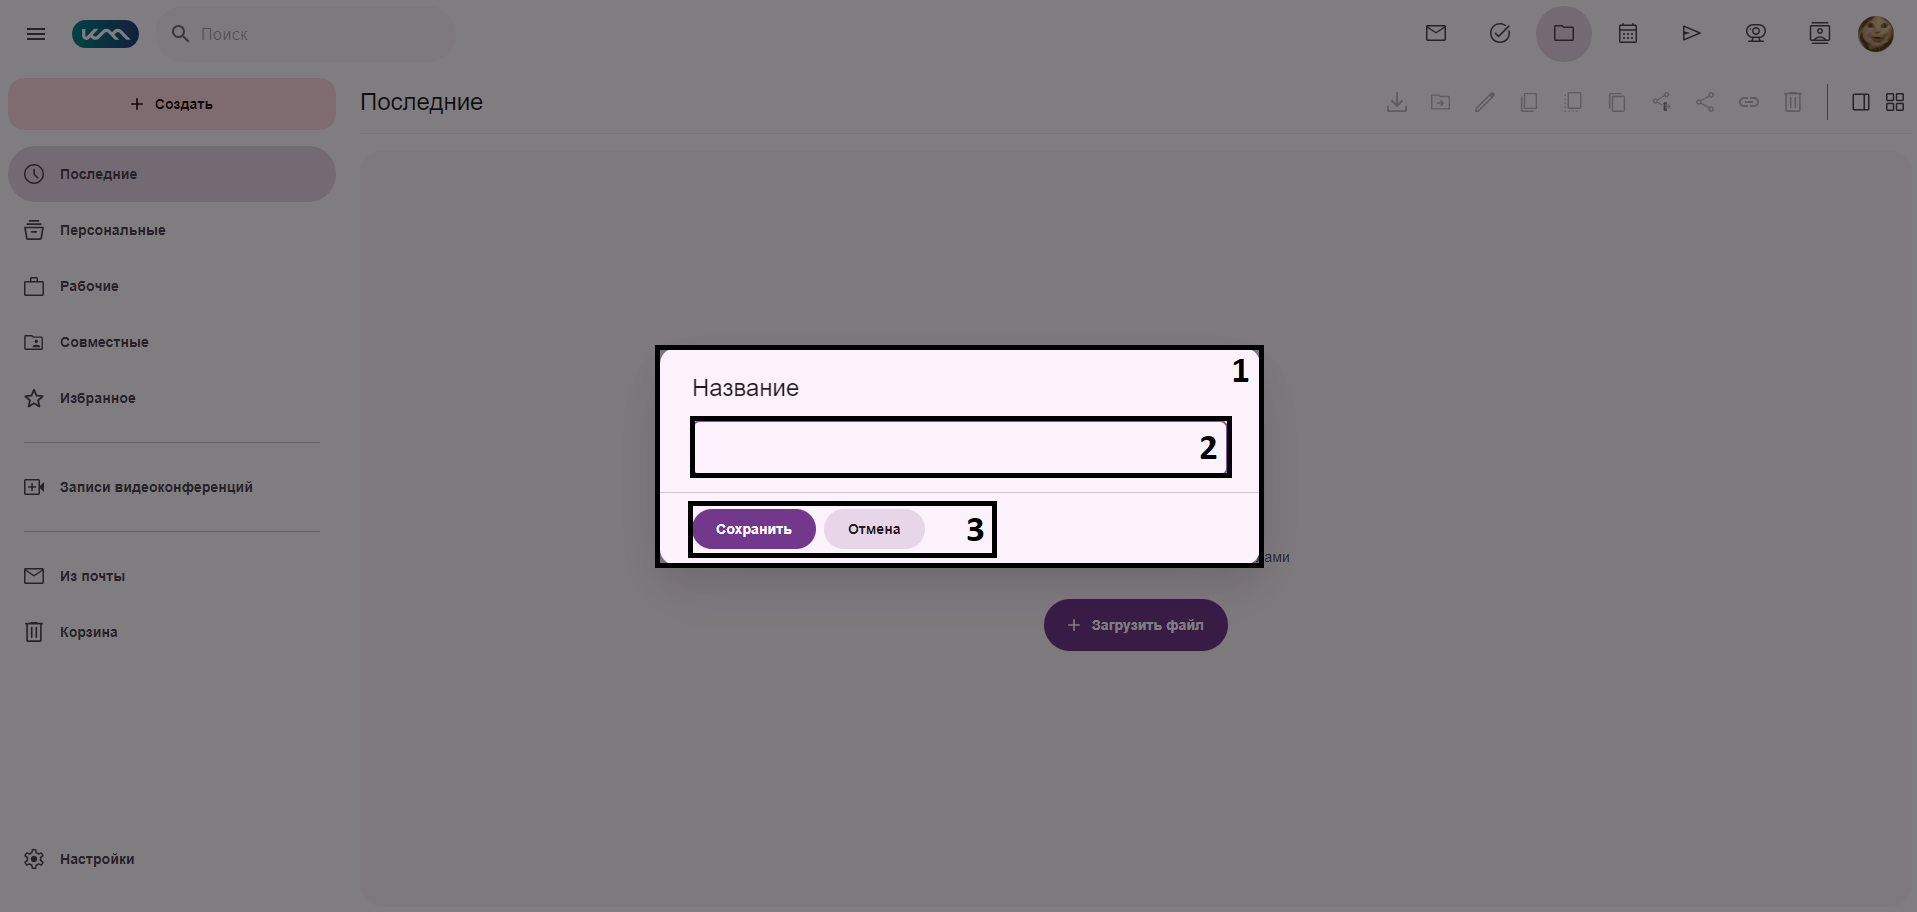
\includegraphics[width=1\linewidth]{images/файлы2}
	\caption{Композиция интерфейса создания файла}
	\label{templ:image9b}
\end{figure}

Композиция интерфейса загрузки файла в сервисе <<Файлы>> представлена на рисунке \ref{templ:image9c} и состоит из:
\begin{itemize}
  \item всплывающего окна (1);
  \item поля для выгрузки файла (2);
  \item кнопок действий (3);
\end{itemize}
\begin{figure}[H]
	\centering
	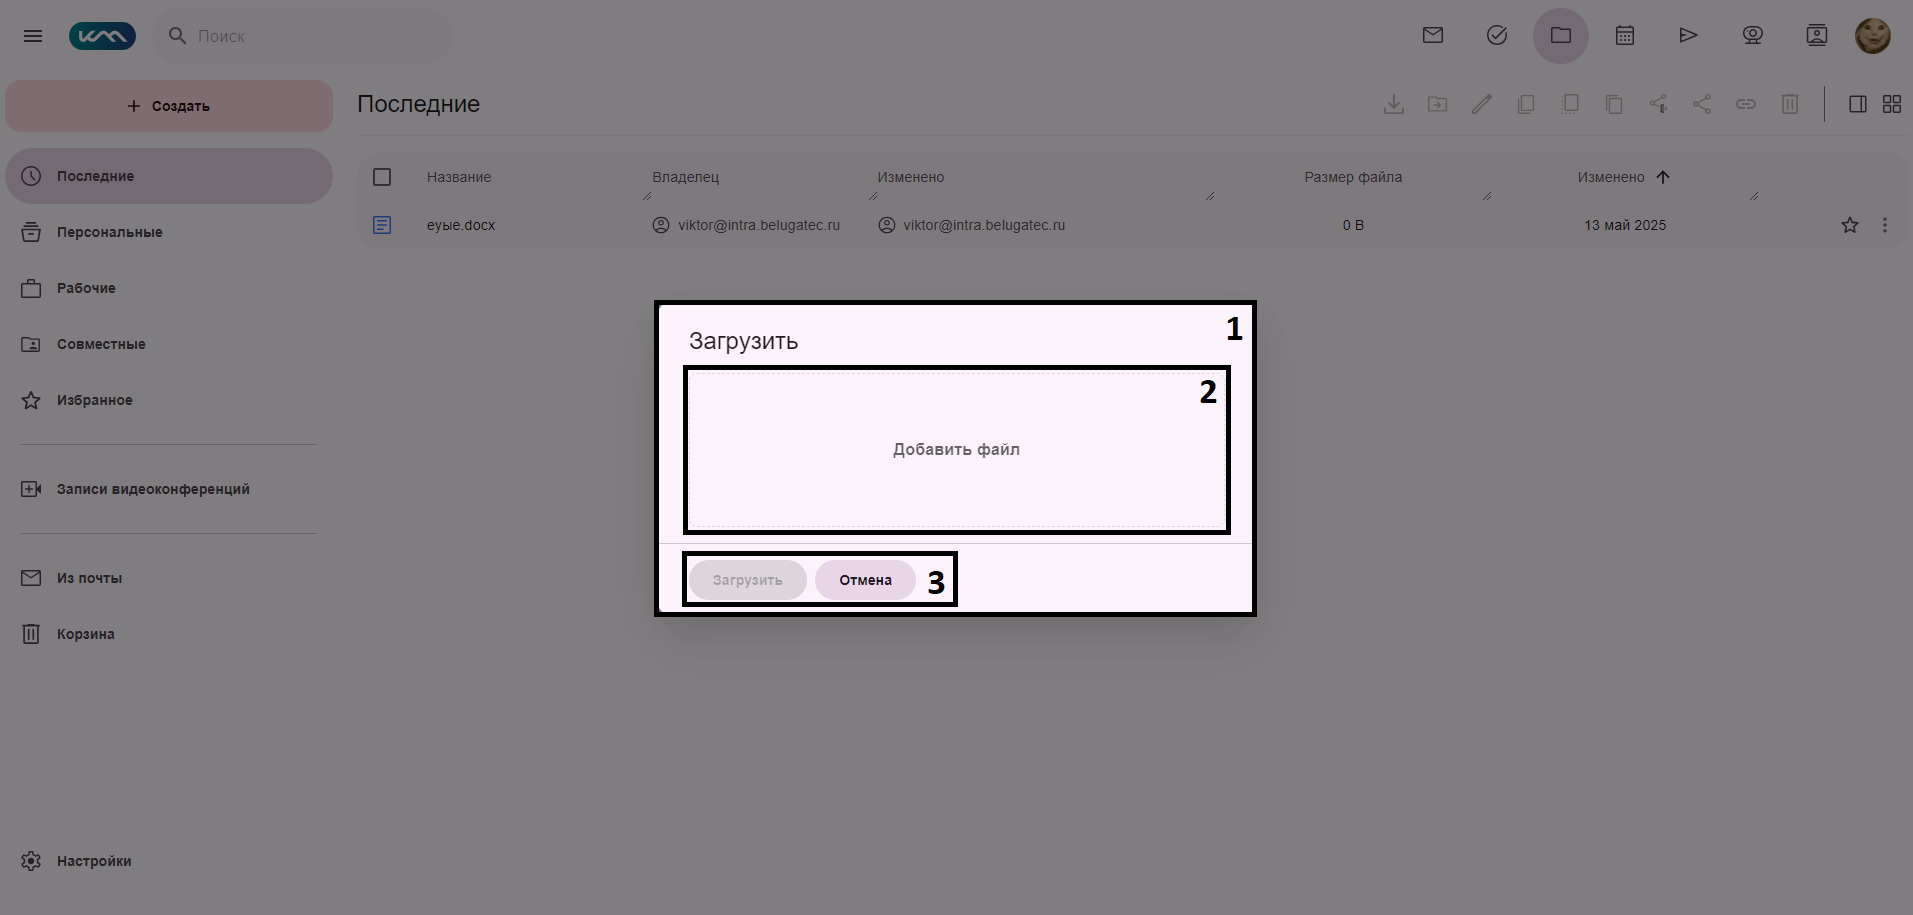
\includegraphics[width=1\linewidth]{images/файлы3}
	\caption{Композиция интерфейса загрузки файла}
	\label{templ:image9c}
\end{figure}

Композиция интерфейса создания папки в сервисе <<Файлы>> представлена на рисунке \ref{templ:image9d} и состоит из:
\begin{itemize}
  \item всплывающего окна (1);
  \item поля названия папки (2);
  \item кнопок действий (3);
\end{itemize}
\begin{figure}[H]
	\centering
	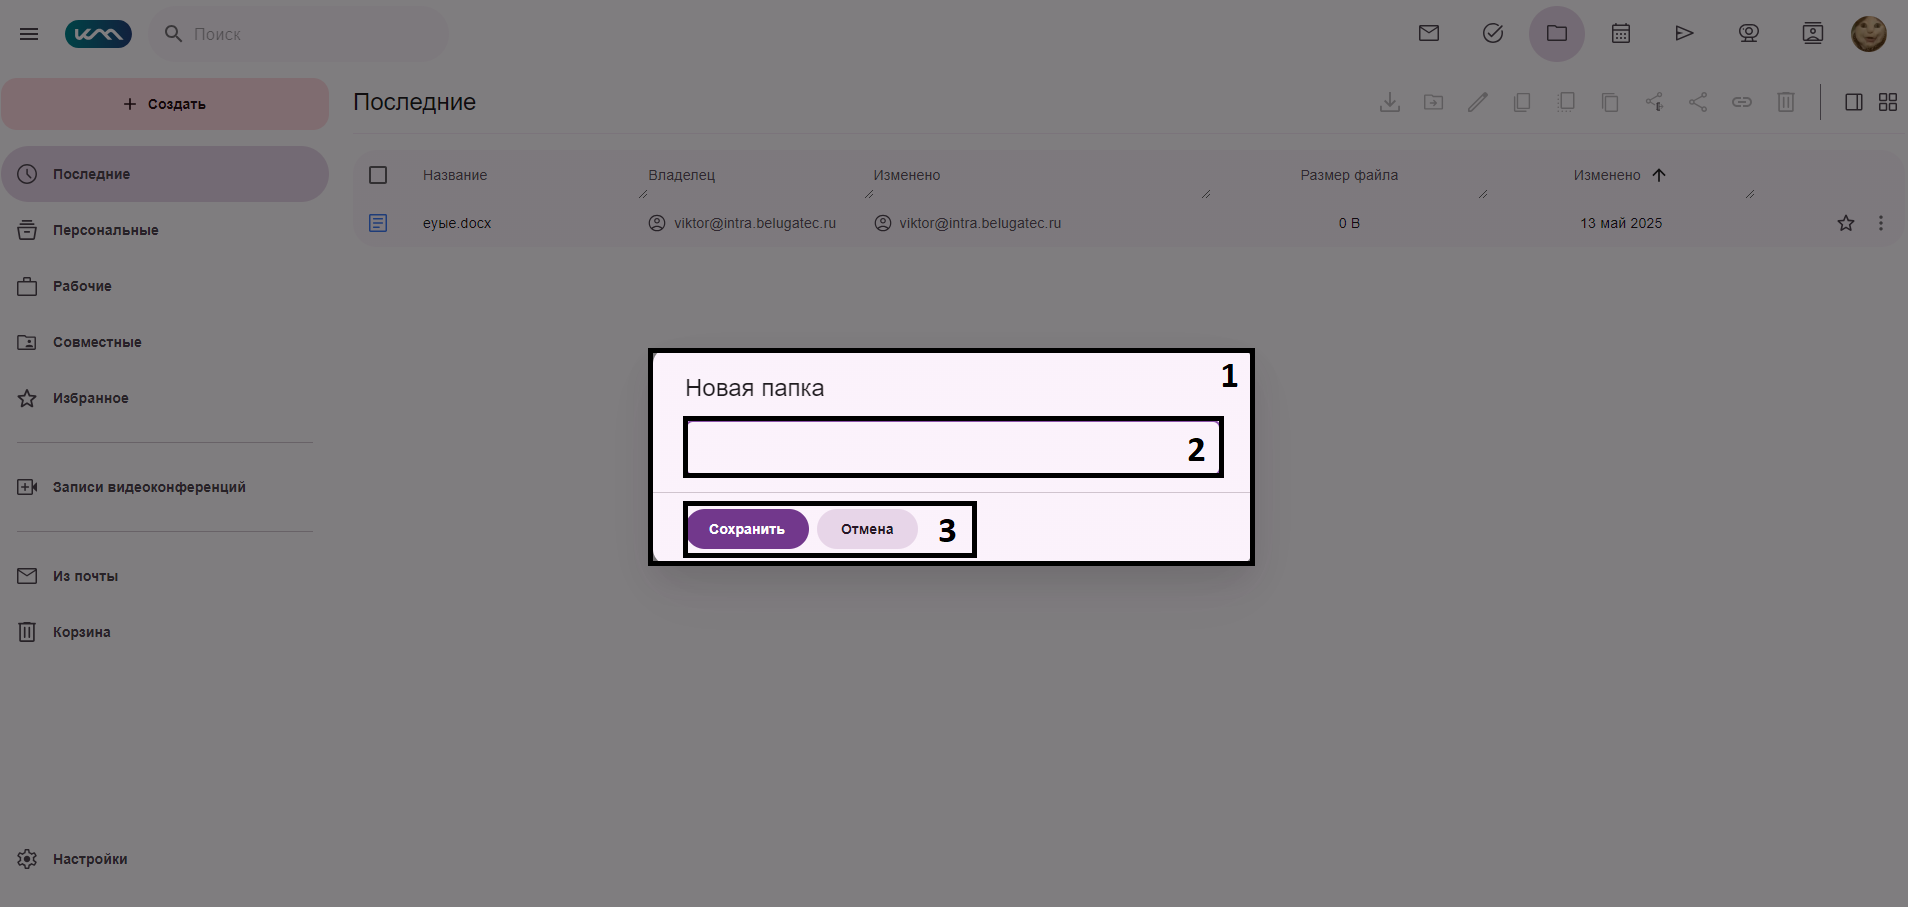
\includegraphics[width=1\linewidth]{images/файлы4}
	\caption{Композиция интерфейса создания папки}
	\label{templ:image9d}
\end{figure}

\clearpage
\subsection{Моделирование вариантов использования}

Для разрабатываемой системы была создана модель, которая демонстрирует способы взаимодействия пользователей с программой с помощью унифицированного языка моделирования UML.

На диаграмме вариантов использования система представлена через набор сценариев (прецедентов), с которыми взаимодействуют актёры — пользователи или внешние компьютерные системы. Каждый вариант использования отображается в виде овала с подписью, обозначающей соответствующий сценарий. Эти сценарии описывают, как пользователь может достичь своих целей, взаимодействуя с функциональностью программы. Взаимосвязь между актёрами и вариантами использования показывается через ассоциации.

Применение UML-диаграмм для визуализации работы системы помогает выявить основные взаимодействия и зависимости между компонентами, что облегчает понимание требований, упрощает проектирование и способствует более качественной разработке и тестированию программного обеспечения.

Пользователь с ролью сотрудника имеет доступ ко всем функциональным модулям веб-платформы:
\begin{itemize}
  \item работа с сервисом <<Почта>>;
  \item работа с сервисом <<Разговоры>>;
  \item работа с сервисом <<Проекты>>;
  \item работа с сервисом <<Календарь>>;
  \item работа с сервисом <<Видеоконференцсвязь>>;
  \item работа с сервисом <<Файлы>>;
  \item работа с сервисом <<Контакты>>;
  \item работа с сервисом <<Настройки>>;
  \item работа с сервисом <<Панель управления>>.
\end{itemize}
Эти действия отображены на диаграмме прецедентов, представленной на рисунке~\ref{templ:actor1}.
\begin{figure}[H]
	\centering
	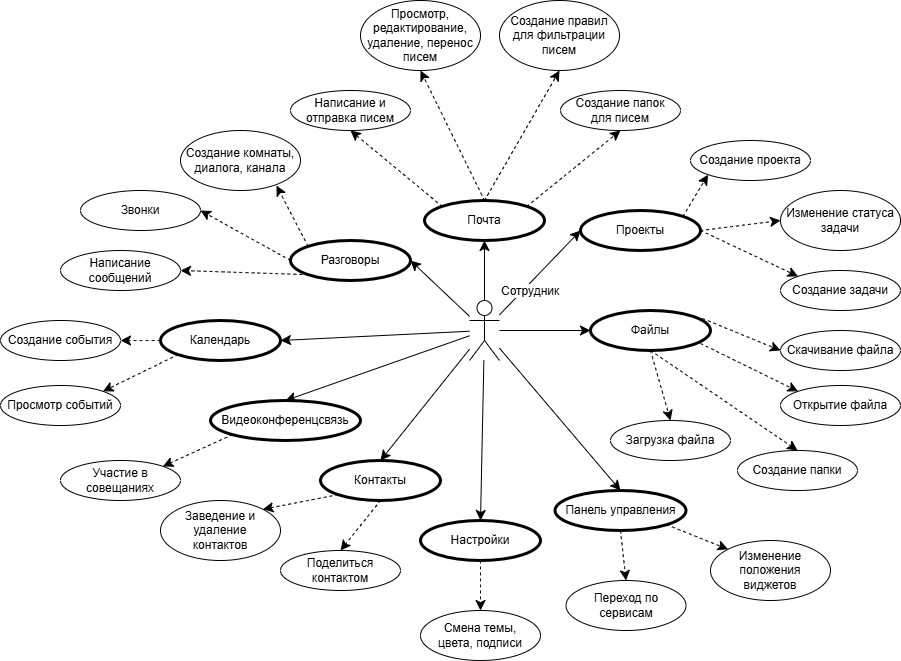
\includegraphics[width=1\linewidth]{images/umldi}
	\caption{Диаграмма прецедентов для сотрудника}
	\label{templ:actor1}
\end{figure}

\subsection{Требования к оформлению документации}

Документация проекта и программного продукта должна оформляться в соответствии с ГОСТ 19.102–77 и ГОСТ 34.601–90. Используемая терминология должна соответствовать принятой в сфере ИТ и быть однозначно понятной.

\section{Технический проект}
\subsection{Общая характеристика организации решения задачи}

Необходимо спроектировать и разработать веб-платформу, направленную на продвижение и оптимизацию деятельности компании на рынке.

Интернет-платформа представляет собой совокупность взаимосвязанных веб-сервисов, доступных через единый пользовательский интерфейс. Каждый сервис представляет собой отдельный функциональный модуль, содержащий текстовую, графическую, а также мультимедийную информацию (видеоконференции, изображения, файлы и т.д.).

Веб-платформа и её веб-сервисы будут размещены в сети Интернет по определённому доменному имени (например, https://calendar.mycompany.ru, https://talks.mycompany.ru, https://mail.mycompany.ru и т.д.). Каждая страница платформы реализуется с использованием современных веб-технологий: HTML, CSS, JavaScript (React) и других, а также может использовать фреймворки и библиотеки для обеспечения адаптивности, интерактивности и высокой производительности.

\subsection{Обоснование выбора технологии проектирования}

На сегодняшний день информационный рынок, поставляющий программные решения в выбранной сфере, предлагает множество продуктов, позволяющих достигнуть поставленной цели – разработки веб-платформы.

\subsubsection{Описание используемых языков программирования}

В процессе разработки веб-платформы используются программные средства и языки программирования. Каждое программное средство и каждый язык программирования применяется для круга задач, при решении которых они необходимы.

\subsubsection{Язык программирования Python}

Python — это высокоуровневый язык программирования общего назначения с поддержкой нескольких парадигм, включая объектно-ориентированное, процедурное и функциональное программирование. Благодаря своей простоте, читаемости и обширной экосистеме библиотек, Python широко применяется в разработке веб-приложений, автоматизации процессов, анализе данных, машинном обучении и многих других областях. В контексте разработки веб-приложений Python используется совместно с фреймворками, такими как Django и Flask, которые обеспечивают удобные средства для создания серверной логики, обработки запросов и генерации динамических веб-страниц.

\subsubsection{Язык программирования JavaScript}

\paragraph{Достоинства языка JavaScript}

JavaScript — это высокоуровневый интерпретируемый язык программирования, основной задачей которого является создание интерактивного поведения на веб-страницах. Он является неотъемлемой частью технологии разработки клиентской части веб-приложений и поддерживается всеми современными веб-браузерами. С помощью JavaScript можно реализовывать динамическое обновление содержимого, проверку данных на стороне клиента, обработку событий, а также взаимодействие с сервером без перезагрузки страницы (через AJAX-запросы). Современные стандарты JavaScript (начиная с ECMAScript 6) предоставляют широкий набор возможностей, включая модули, асинхронные функции, классы и работу с промисами. Для повышения совместимости и ускорения разработки часто используются библиотеки и фреймворки, такие как jQuery, React, Vue.js и другие. Они позволяют упростить доступ к элементам DOM, реализовать реактивные интерфейсы и обеспечить кроссбраузерную поддержку. JavaScript выполняется непосредственно в браузере пользователя, что позволяет создавать отзывчивые и интерактивные пользовательские интерфейсы без необходимости постоянной связи с сервером.

\paragraph{Недостатки языка JavaScript}

\begin{itemize}
  \item parseInt("08") // → 0
  \item parseInt("0x10") // → 16
  \item parseInt("0x10", 10) // → 0
  \item null == 0 // → false
  \item null > 0 // → false
  \item null >= 0 // → true
  \item undefined == null // → true
  \item undefined === null // → false
  \item typeof NaN // → "number"
  \item NaN === NaN // → false
  \item "5" + 3 // → "53"
  \item "5" - 3 // → 2
  \item "5" * "3" // → 15
  \item "5" * "abc" // → NaN
  \item 0.1 + 0.2 === 0.3 // → false
  \item (0.1 + 0.2).toFixed(1) // → "0.3"
  \item true + true // → 2
  \item true - false // → 1
  \item "1" + true // → "1true"
  \item "1" - true // → 0
\end{itemize}

\subsubsection{React}
React — это популярная JavaScript-библиотека для создания пользовательских интерфейсов. Она позволяет строить интерактивные веб-приложения с помощью компонентного подхода.

Основные преимущества React:
\begin{itemize}
\item Виртуальный DOM для эффективного обновления интерфейса
\item Компонентная архитектура, способствующая повторному использованию кода
\item Односторонний поток данных, упрощающий отладку приложений
\item Богатая экосистема дополнительных библиотек и инструментов
\item Поддержка серверного рендеринга (Next.js)
\end{itemize}

В нашем проекте React используется для построения клиентской части всех веб-сервисов платформы. Это позволяет создавать единообразные, отзывчивые интерфейсы с высокой производительностью.

\subsubsection{Apache James и JMAP}
Apache James — это open-source почтовый сервер, написанный на Java. Он предоставляет полный набор почтовых протоколов (SMTP, POP3, IMAP) и может использоваться как самостоятельное решение или как часть более крупной системы.

JMAP (JSON Meta Application Protocol) — современный протокол для работы с почтой, календарями и контактами, призванный заменить устаревшие IMAP и SMTP. Его преимущества:
\begin{itemize}
\item Использование JSON для передачи данных
\item Эффективная синхронизация состояния
\item Поддержка push-уведомлений
\item Единый API для почты, календарей и контактов
\end{itemize}

В нашей платформе мы используем Apache James с поддержкой JMAP для реализации почтового сервиса, что обеспечивает:
\begin{itemize}
\item Надежную доставку и хранение почты
\item Быструю синхронизацию между клиентами
\item Современный API для интеграции с другими сервисами
\end{itemize}

\subsubsection{Node.js}
Node.js — это серверная платформа для выполнения JavaScript, построенная на движке V8. Она использует событийно-ориентированную, неблокирующую модель ввода-вывода, что делает её легковесной и эффективной.

Основные особенности Node.js, используемые в нашем проекте:
\begin{itemize}
\item Высокая производительность для I/O-интенсивных операций
\item Единая языковая среда для клиента и сервера (JavaScript)
\item Богатая экосистема пакетов (npm)
\item Поддержка современных стандартов JavaScript
\end{itemize}

В нашей архитектуре Node.js используется для:
\begin{itemize}
\item Реализации серверной логики некоторых микросервисов
\item Обработки реального времени (чаты, уведомления)
\item Серверного рендеринга React-приложений
\item Построения API-шлюза для объединения различных сервисов
\end{itemize}

Сочетание этих технологий позволяет нам создать масштабируемую, производительную платформу с современным пользовательским интерфейсом и надежной серверной частью.

\subsection{Диаграмма компонентов}

Диаграмма компонентов отображает взаимодействие пользователя с сервисами. Основными элементами диаграммы являются компоненты (сервисы).

\begin{figure}[H]
\center{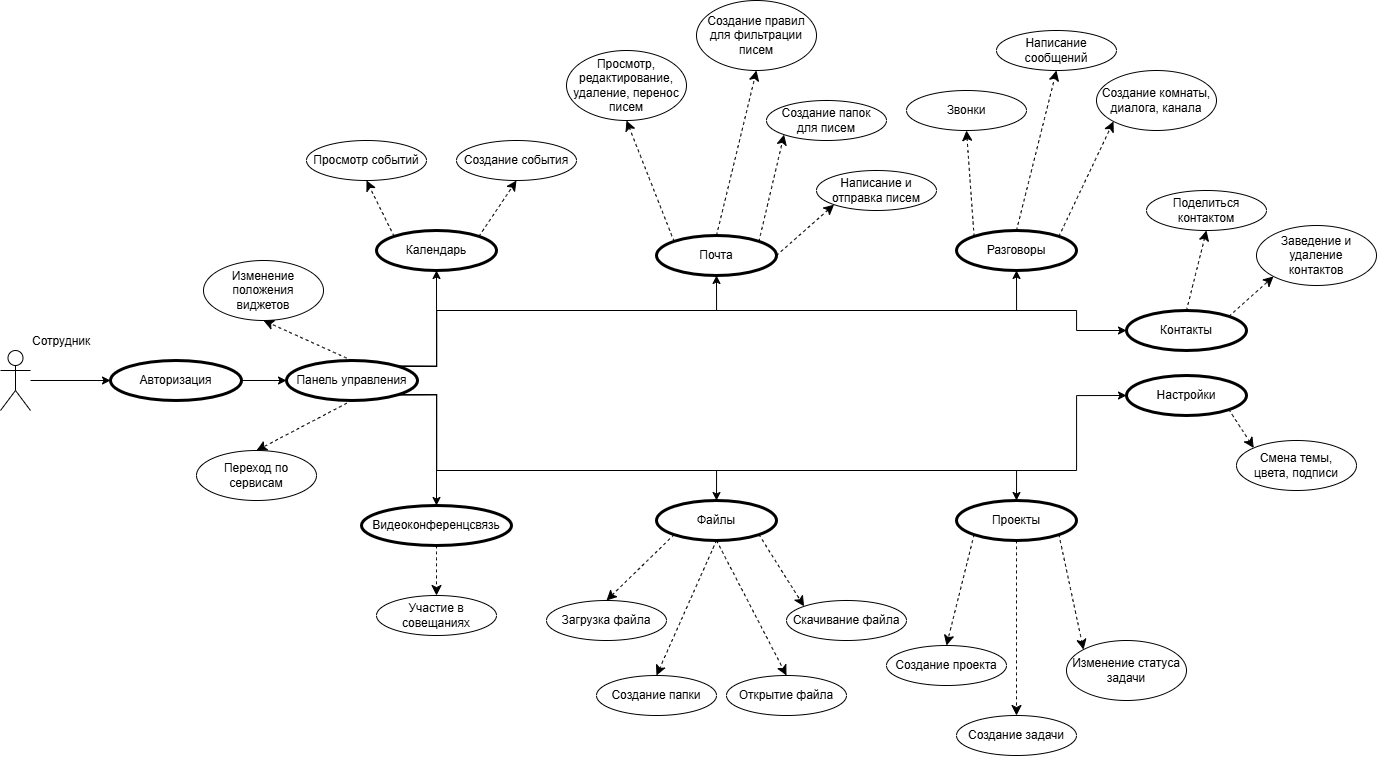
\includegraphics[width=1\linewidth]{images/diag2}}
\caption{Диаграмма компонентов}
\label{comp:image}
\end{figure}

После авторизации в веб-платформе пользователь переходит на главную рабочую страницу <<Панель управления>>, где отображаются виджеты различных сервисов, в которые он может перейти и работать с ними напрямую.

\begin{itemize}
    \item Сервис <<Почта>> — пользователь может просматривать свои письма, отвечать на них, а также отправлять новые письма. В сервисе отображаются последние 10 входящих писем из папки Входящие. Пользователь может выбрать получателя из списка контактов и отправить письмо. Также сервис интегрирован с функцией звонков, и при наличии соответствующей кнопки в письме пользователь может совершить звонок через сервис <<Разговоры>>.
    
    \item Сервис <<Файлы>> — в этом сервисе пользователь может загружать, хранить и управлять своими файлами. Он может поделиться файлами с другими пользователями, выбрав их из списка контактов. Пользователь может настраивать права доступа для каждого файла, например, на скачивание или редактирование.

    \item Сервис <<Контакты>> — сервис предоставляет пользователю возможность управлять списком своих контактов. Он может быстро находить пользователей для отправки писем, звонков или назначения задач. В сервисе можно просматривать информацию о контактах, включая их статус и доступные способы связи.

    \item Сервис <<Разговоры>> — этот сервис позволяет пользователю совершать голосовые или видеозвонки с людьми из списка контактов. Пользователь может выбрать способ связи (текстовый чат, голосовой или видеозвонок) и начать общение. Сервис интегрируется с почтовым сервисом, позволяя удобно начинать звонки после переписки по почте.

    \item Сервис <<Задачи>> — в этом сервисе пользователь может назначать задачи другим пользователям, выбрав их из списка контактов. Задачи могут быть связаны с проектами или обычными делами. Пользователь может отслеживать состояние задач (выполнена, в процессе и т.д.) и получать уведомления о статусе задач.

    \item Сервис <<Видеоконференцсвязь>> — в этом сервисе пользователь может создавать или присоединяться к видеоконференциям. Он может приглашать участников, проводить видеозвонки и использовать функции обмена экранами и чатом во время конференции.

    \item Сервис <<Календарь>> — сервис календаря позволяет пользователю планировать свои события и задачи. Пользователь может добавлять мероприятия, настраивать напоминания и получать уведомления о предстоящих событиях. Календарь интегрируется с задачами, и пользователь может добавлять задачи в календарь для более удобного планирования.

    \item Сервис <<Настройки>> — в этом сервисе пользователь может настроить параметры своей учетной записи, такие как изменение личной информации, настройка уведомлений, конфиденциальности и безопасности. Также можно выбрать тему оформления интерфейса (светлая или темная) и язык платформы.
\end{itemize}

\subsection{Диаграмма размещения}

Диаграмма размещения (рис.~\ref{place:image}) отражает физические взаимосвязи между программными и аппаратными компонентами системы.

\vspace{-8mm} % чтобы убрать пустую строку, которая осталась после переноса рисунка на следующую страницу
\begin{figure}[H]
\center{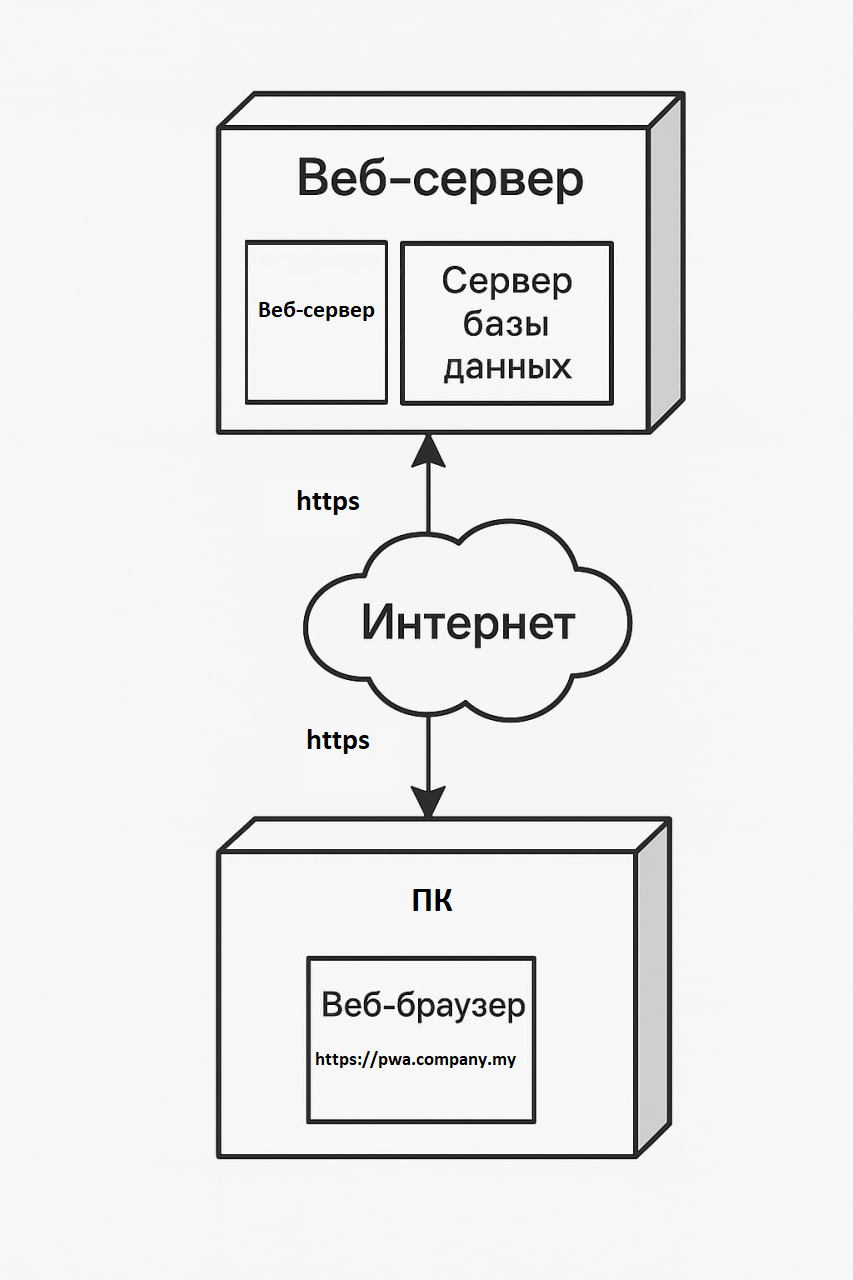
\includegraphics[width=0.57\linewidth]{images/диаграмма2}}
\caption{Диаграмма размещения}
\label{place:image}
\end{figure}

\subsection{Содержание информационных блоков. Основные сущности}

Проанализировав требования, можно выделить следующие основные сущности:
\begin{itemize}
  \item "<Письмо">;
  \item "<Комната видеоконференцсвязи">;
  \item "<Событие календаря">;
  \item "<Виджет">;
  \item "<Контакт">;
  \item "<Настройки">;
  \item "<Проект">;
  \item "<Канал">;
  \item "<Файл">.
\end{itemize}

В состав сущностей входят следующие атрибуты:

\begin{xltabular}{\textwidth}{|l|l|p{3.2cm}|X|}
  \caption{Атрибуты сущности "<Письмо">\label{mail:table}}\\ \hline
  Поле & Тип & Обязательное & Описание \\ \hline
  \endfirsthead
  \continuecaption{Продолжение таблицы \ref{mail:table}}\\ \hline
  Поле & Тип & Обязательное & Описание \\ \hline
  \endhead
  id & ObjectId & true & Уникальный идентификатор письма \\ \hline
  sender & String & true & Отправитель \\ \hline
  recipients & Array[String] & true & Получатели \\ \hline
  subject & String & false & Тема письма \\ \hline
  body & String & false & Текст письма \\ \hline
  attachments & Array & false & Список вложений \\ \hline
  timestamp & Date & true & Дата и время отправки \\ \hline
  read & Boolean & true & Признак прочтения \\ \hline
\end{xltabular}

\begin{xltabular}{\textwidth}{|l|l|p{3.2cm}|X|}
  \caption{Атрибуты сущности "<Комната видеоконференцсвязи">\label{video:table}}\\ \hline
  Поле & Тип & Обязательное & Описание \\ \hline
  \endfirsthead
  \continuecaption{Продолжение таблицы \ref{video:table}}\\ \hline
  Поле & Тип & Обязательное & Описание \\ \hline
  \endhead
  id & ObjectId & true & Уникальный идентификатор конференции \\ \hline
  participants & Array[String] & true & Участники \\ \hline
  startTime & DateTime & true & Время начала \\ \hline
  endTime & DateTime & false & Время окончания \\ \hline
  status & String & true & Статус (запланирована, активна, завершена) \\ \hline
\end{xltabular}

\begin{xltabular}{\textwidth}{|l|l|p{3.2cm}|X|}
  \caption{Атрибуты сущности "<Событие календаря">\label{calendar:table}}\\ \hline
  Поле & Тип & Обязательное & Описание \\ \hline
  \endfirsthead
  \continuecaption{Продолжение таблицы \ref{calendar:table}}\\ \hline
  Поле & Тип & Обязательное & Описание \\ \hline
  \endhead
  id & ObjectId & true & Уникальный идентификатор события \\ \hline
  title & String & true & Название события \\ \hline
  date & DateTime & true & Дата и время \\ \hline
  participants & Array[String] & false & Участники \\ \hline
  description & String & false & Описание \\ \hline
\end{xltabular}

\begin{xltabular}{\textwidth}{|l|l|p{3.2cm}|X|}
  \caption{Атрибуты сущности "<Виджет">\label{dashboard:table}}\\ \hline
  Поле & Тип & Обязательное & Описание \\ \hline
  \endfirsthead
  \continuecaption{Продолжение таблицы \ref{dashboard:table}}\\ \hline
  Поле & Тип & Обязательное & Описание \\ \hline
  \endhead
  id & ObjectId & true & Идентификатор виджета \\ \hline
  name & String & true & Название виджета \\ \hline
  type & String & true & Тип виджета (статистика, список задач и т.д.) \\ \hline
  dataSource & String & true & Источник данных \\ \hline
\end{xltabular}

\begin{xltabular}{\textwidth}{|l|l|p{3.2cm}|X|}
  \caption{Атрибуты сущности "<Контакт">\label{contacts:table}}\\ \hline
  Поле & Тип & Обязательное & Описание \\ \hline
  \endfirsthead
  \continuecaption{Продолжение таблицы \ref{contacts:table}}\\ \hline
  Поле & Тип & Обязательное & Описание \\ \hline
  \endhead
  id & ObjectId & true & Уникальный идентификатор контакта \\ \hline
  name & String & true & Имя контакта \\ \hline
  email & String & true & Email \\ \hline
  phone & String & false & Телефон \\ \hline
  tags & Array[String] & false & Метки \\ \hline
\end{xltabular}

\begin{xltabular}{\textwidth}{|l|l|p{3.2cm}|X|}
  \caption{Атрибуты сущности "<Настройки">\label{settings:table}}\\ \hline
  Поле & Тип & Обязательное & Описание \\ \hline
  \endfirsthead
  \continuecaption{Продолжение таблицы \ref{settings:table}}\\ \hline
  Поле & Тип & Обязательное & Описание \\ \hline
  \endhead
  id & ObjectId & true & Идентификатор настройки \\ \hline
  userId & ObjectId & true & Пользователь \\ \hline
  theme & String & false & Выбранная тема \\ \hline
  language & String & false & Язык интерфейса \\ \hline
\end{xltabular}

\begin{xltabular}{\textwidth}{|l|l|p{3.2cm}|X|}
  \caption{Атрибуты сущности "<Проект">\label{projects:table}}\\ \hline
  Поле & Тип & Обязательное & Описание \\ \hline
  \endfirsthead
  \continuecaption{Продолжение таблицы \ref{projects:table}}\\ \hline
  Поле & Тип & Обязательное & Описание \\ \hline
  \endhead
  id & ObjectId & true & Идентификатор проекта \\ \hline
  title & String & true & Название проекта \\ \hline
  description & String & false & Описание \\ \hline
  members & Array[String] & true & Участники проекта \\ \hline
  status & String & true & Текущий статус \\ \hline
\end{xltabular}

\begin{xltabular}{\textwidth}{|l|l|p{3.2cm}|X|}
  \caption{Атрибуты сущности "<Канал">\label{talks:table}}\\ \hline
  Поле & Тип & Обязательное & Описание \\ \hline
  \endfirsthead
  \continuecaption{Продолжение таблицы \ref{talks:table}}\\ \hline
  Поле & Тип & Обязательное & Описание \\ \hline
  \endhead
  id & ObjectId & true & Идентификатор беседы \\ \hline
  participants & Array[String] & true & Участники \\ \hline
  messages & Array & true & Сообщения \\ \hline
  lastMessage & String & false & Последнее сообщение \\ \hline
  unreadCount & Integer & true & Количество непрочитанных \\ \hline
\end{xltabular}

\begin{xltabular}{\textwidth}{|l|l|p{3.2cm}|X|}
  \caption{Атрибуты сущности "<Файл">\label{files:table}}\\ \hline
  Поле & Тип & Обязательное & Описание \\ \hline
  \endfirsthead
  \continuecaption{Продолжение таблицы \ref{files:table}}\\ \hline
  Поле & Тип & Обязательное & Описание \\ \hline
  \endhead
  id & ObjectId & true & Идентификатор файла \\ \hline
  name & String & true & Название файла \\ \hline
  owner & String & true & Владелец \\ \hline
  sharedWith & Array[String] & false & Список, с кем поделились \\ \hline
  size & Integer & true & Размер в байтах \\ \hline
  createdAt & Date & true & Дата загрузки \\ \hline
\end{xltabular}

Экземпляры этих сущностей реализуются в информационных блоках пользовательского интерфейса. Атрибуты сущностей отображаются в полях, свойствах и компонентах соответствующих элементов.

\ifПрактика{}\else{
   \input{РабочийПроект}
   \input{Заключение}
}\fi
\addcontentsline{toc}{section}{СПИСОК ИСПОЛЬЗОВАННЫХ ИСТОЧНИКОВ}

\begin{thebibliography}{9}

    \bibitem{react3} Бэнкс А., Порселло Е. React и Redux. Функциональная веб-разработка. — СПб.: Питер, 2018. — 336 с. — ISBN 978-5-4461-0669-1. — Текст: непосредственный.

    \bibitem{htmlcss} Дэкетт Д. HTML и CSS. Разработка и создание веб-сайтов. — М.: Эксмо, 2014. — 480 с. — ISBN 978-5-699-64193-2. — Текст: непосредственный.

    \bibitem{javascript1} Флэнаган Д. JavaScript. Подробное руководство. — М.: Вильямс, 2020. — 960 с. — ISBN 978-5-8459-1904-5. — Текст: непосредственный.

    \bibitem{python3} Матей Н. Python. К вершинам мастерства. — СПб.: Питер, 2022. — 432 с. — ISBN 978-5-4461-0926-5. — Текст: непосредственный.

    \bibitem{javascript2} Марейн М. Выразительный JavaScript. — СПб.: Питер, 2020. — 472 с. — ISBN 978-5-4461-1188-6. — Текст: непосредственный.

    \bibitem{python1} Лутц М. Изучаем Python. — 5-е изд. — СПб.: Питер, 2021. — 1300 с. — ISBN 978-5-4461-1556-3. — Текст: непосредственный.

    \bibitem{python2} Свигарт А. Автоматизация рутинных задач с помощью Python. — 2-е изд. — СПб.: Питер, 2021. — 592 с. — ISBN 978-5-4461-1865-6. — Текст: непосредственный.

    \bibitem{react2} Вайс А. React в действии. — СПб.: Питер, 2019. — 384 с. — ISBN 978-5-4461-1091-9. — Текст: непосредственный.

    \bibitem{css1} Веру Л. CSS-секреты. 47 советов по улучшению веб-интерфейсов. — СПб.: Питер, 2017. — 368 с. — ISBN 978-5-496-02699-4. — Текст: непосредственный.

    \bibitem{css2} Юэнс В. CSS. Карманный справочник. — М.: Символ-Плюс, 2020. — 272 с. — ISBN 978-5-93286-362-0. — Текст: непосредственный.

\end{thebibliography}
\ifВКР{\input{Плакаты}}\fi
\ifПрактика{}\else{\input{Код}}\fi
\end{document}
